\documentclass[12pt, a4paper,titlepage]{article}
\usepackage[utf8]{inputenc}
\usepackage[english, swedish]{babel}
\usepackage{graphicx} 
\usepackage{titling}
\graphicspath{{bilder/}}
\usepackage{minted} %kod
\usepackage{mathptmx} %font
\usepackage{hanging}
\usepackage{xurl}
\usepackage{subcaption} 
\usepackage[hidelinks]{hyperref}
\renewcommand{\familydefault}{\sfdefault}




\setlength{\droptitle}{-15em}
\title{
\begin{minipage}{0.4\textwidth}

\includegraphics[width=\linewidth]{SSIS-logo(1).png}
\end{minipage}%
\hfill%
\begin{minipage}{0.6\textwidth}\raggedleft
\normalsize{Stockholm Science \& Innovation School
\\Gymnasiearbete
\\Handledare: Sandra Forsman}
\end{minipage}
\\[25ex]\Huge{Proi Exypno}\\{\large Den frågvisa väckarklockan}}
\author{\LARGE{Sam Shahriari}}
\date{}


\begin{document}

    \maketitle
    \selectlanguage{english}
    \begin{abstract}
    \addcontentsline{toc}{section}{Abstract}
    The aim of this project was to build an alarm clock that makes sure that we go up when the alarm rings and to investigate how a smart alarm clock is built. The prototype of the alarm clock was based on the microcomputer Raspberry~Pi~3. It printed information to the user with an LCD-screen and received input from push buttons. The computer code was written in the language Python~2. When the alarm clock rings, a question is showed at the display. In order to turn the alarm off, the question must be correctly answered. The discussion addresses why the components were chosen and how the code works. The report ends with ideas for improvement. These are to solder all the components to a PCB, create a case and to add more and different types of questions.

    \end{abstract}

    \selectlanguage{swedish}
    \tableofcontents
    \thispagestyle{empty}
    \newpage

    \setcounter{page}{3}
    
   % \section{Förord}
    %Tack:
o	Sandra
o	Alla som testat
o	Guiden
o	Alex 
o	Serkan
o	Alla lärare 

    %\newpage
    
    \section{Introduktion}
    \subsection{Bakgrund}
Idag är det många som väcks av ett alarm på morgonen. Antingen av en väckar\-klocka eller en mobiltelefon. Av de som använder alarm är det ungefär hälften som använder {snooze-knappen} (Roitmann, 2017). När knappen trycks ner tystnar larmet och ringer igen efter ett antal minuter. Enligt Torbjörn Åkerstedt, sömnforskare på Karolinska Institutet, kan snoozningen göra att man blir ännu trögare när man vaknar en andra gång (TT, 2013).

För att lösa denna problematik med att folk snoozar istället för att gå upp finns det i dagsläget flera olika typer av alarmklockor. Det finns klockor som skjuter iväg föremål som användaren måste finna, klockor som gömmer sig och klockor som stängs av efter genomfört pussel (BoredPanda, 2011). 
\subsection{Syfte}
Syftet med projektet var att göra en väckarklocka som ser till att användaren verkligen går upp på morgonen. %Detta åstadkomms genom att väckarklockan saknar en snooze-knapp och alarmet stängs inte av förrän en klarar av att svara korrekt vilket en måste vakna för. (denna mening kommer att skrivas om och delas upp)
 
 \subsection{Frågeställningar}
\begin{itemize}
    \item {Hur skapas en smart väckarklocka?}
    \item {Hur ska en väckarklocka se till att vi verkligen går upp?}
    %\item {Hur hjälper en väckarklocka i vardagen?}
\end{itemize}

\subsection{Mål}
Målet är att skapa en väckarklocka som ser till att personen går upp när klockan ringer genom att användaren måste besvara en fråga för att tysta alarmet. Det ska vara lätt att kunna lägga till nya frågor och det ska vara intuitiva kontroller för användaren, exempelvis att ställa in alarmtiden och besvara frågor. 


    %\newpage
    
    \section{Genomförande}
    %\subsection{Materiel}
%LCD-skärm(16x02), högtalare, kablar, Kicad, knappar, kopplingsdäck, potentiometrar, Putty, Raspberry Pi 3 \& resistorer.

%\subsection{Metod}
I första steget skedde allt förarbete inklusive planeringen. \hyperref[sec:svar]{En enkät skickades ut angående önskemål om väckarklockan} och typ av enkortsdator valdes.

En översikt av alla önskade funktioner skapades som \hyperref[sec:psuedo]{pseudokod}. Därefter skrevs programmet och frågor. En prototyp skapades och kopplingen skissades%knappar, display och dylikt kopplades in till enkortsdatorn med hjälp av ett kopplingsdäck
. Slutligen genomfördes test av väckarklockans funktioner.
   
    %\newpage

    \section{Resultat av projektet}
    \subsection{Enkät}
Enkäten besvarades av 172 personer. En majoritet av de svarande föredrar en väckarklocka som visar datum men inte sekunder. Den mest önskade färgen för väckarklockans skal är svart. För fullständiga svar, se \hyperref[sec:svar]{bilaga 6.1}.

%\subsection{Önskade funktioner}
%slå kansek ihop med punkt efter

\subsection{Prototyp}
    Prototypen av väckarklockan grundades på enkortsdatorn Raspberry~Pi~3. Kopplingen kopplades på ett kopplingsdäck. Information visas på en LCD-skärm som kan visa 32 tecken fördelade på två rader. Tre knappar är kopplade till datorn vilket motsvarar $+$, $-$ och $\triangleright$. Andra komponenter är en extern högtalare, potientiometrar för att justera displayens ljusstyrka, resistorer och kablar. Se figur 1 för kopplingen av prototypen och figur 2 för ett kopplingschema över kretsen. För större schema, se \hyperref[sec:krets]{bilaga 6.2}.
    \begin{figure}[h!]
    \centering

        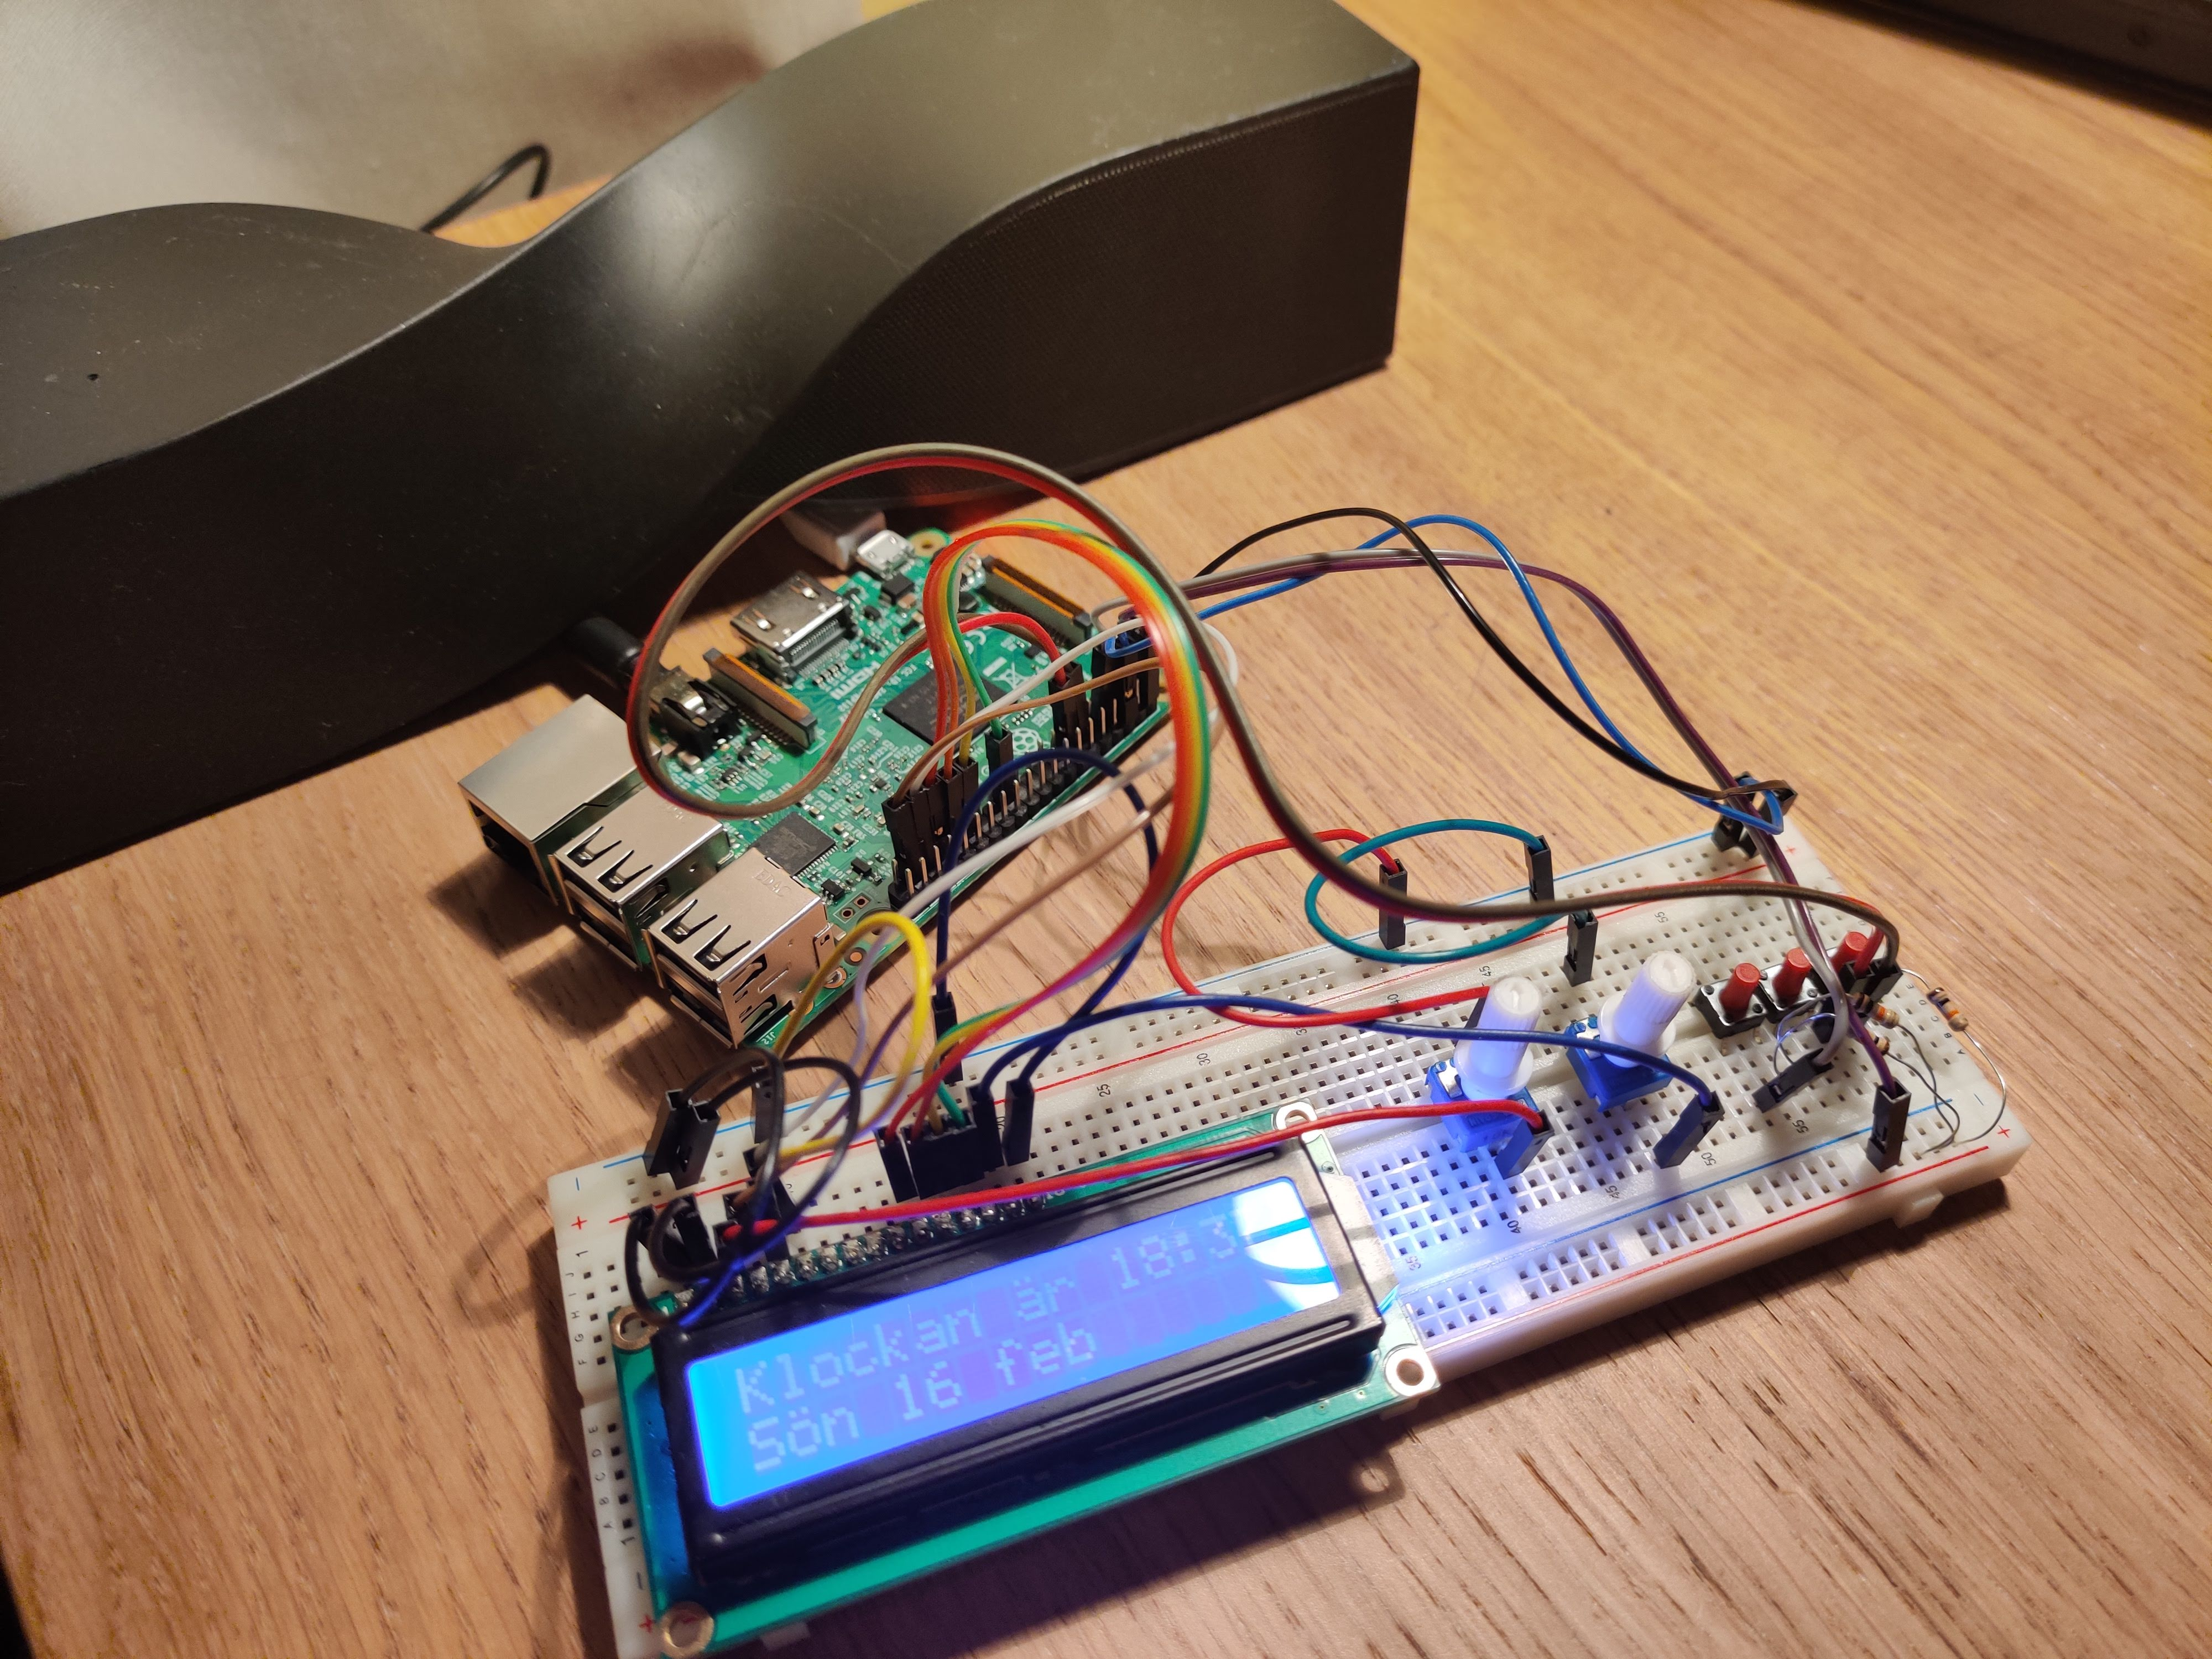
\includegraphics[width=0.4\textwidth]{bilder/koppling.jpg} % first figure itself
        \caption{Kopplingen av protoypen}
    \end{figure}
    \begin{figure}[h!]
    \centering
        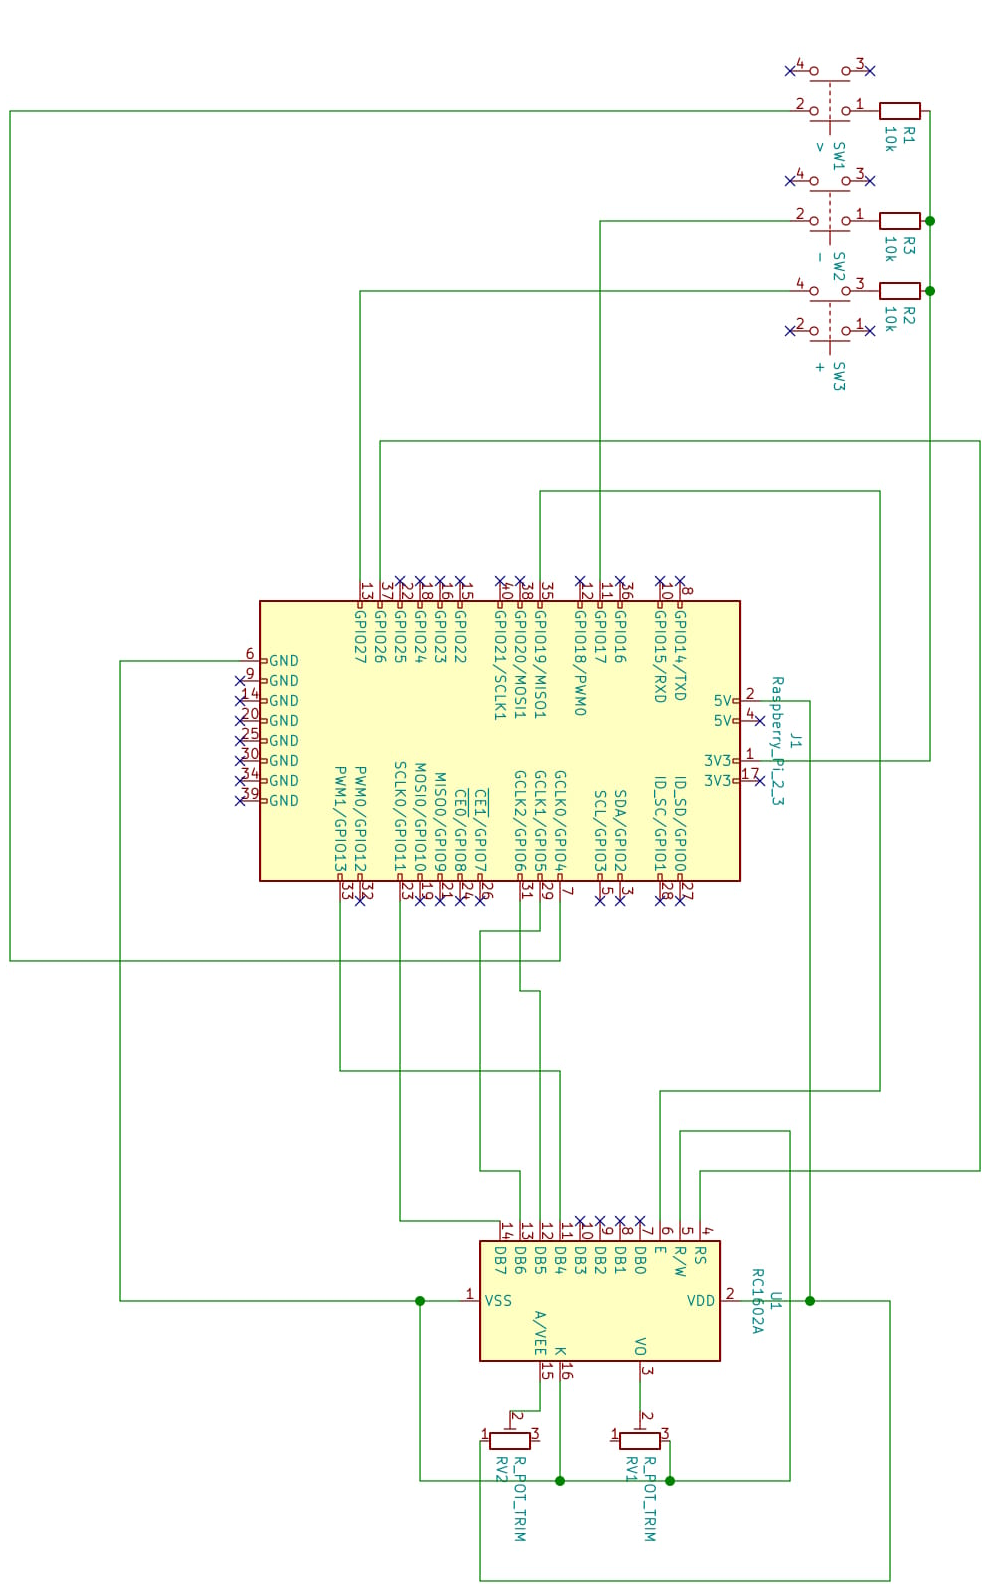
\includegraphics[width=0.35\textwidth,angle=90]{bilder/krets2.png} % second figure itself
        \caption{Kopplingschema}
    \end{figure}

\subsection{Program}
Programmet för väckarklockan är skrivet i programmeringsspråket \emph{Python} version 2.7 och LCD-bibliotek \texttt{CHARLcd} ligger som grund för användar\-kommunikation. Väckarklockans program låter användaren ställa in önskad alarmtid (figur 3) och därefter välja ifall alarmet ska ringa eller inte. När alarmet ringer spelas ljud från en ljudfil upp på repetition tills användaren svarar rätt på en fråga. 

När $\triangleright$ trycks in anropas metoden \verb|alarmvisning| och den tidigare inställda alarmtiden visas. Först ställs timmarna in och därefter minuterna. Alarmtiden kan ställas in i intervall om fem minuter. 

För att  inte tiden ska kunna understiga 00:00 respektive överstiga 23:55 används 
\small{\mint{python}|if (GPIO.input(13) == GPIO.HIGH and alarmH<23 and raknareAlarm==0):| }
\normalsize \noindent och andra liknande if-satser. Variabeln \verb|raknareAlarm| håller reda på ifall det är timmarna eller minuterna som ska ställas in. Ifall \verb|raknareAlarm| är 0 ställs timmarna in, vid 1 ställs minuterna. 

Varje minut uppdateras skärmen med den nya tiden. Detta sker genom att varje gång \mintinline{python}{time.strftime("\%S")} (hämtning av sekunderna) är lika med 0 anropas metoden \texttt{tidsvisning}. 
\begin{minted}[fontsize=\footnotesize]{python}
def tidsvisning():
    lcd.cursor_mode="hide"
    lcd.clear()
    lcd.cursor_pos = (0,0)
    lcd.write_string("Klockan %sr %s" %(unichr(1), time.strftime("%H:%M")))
    lcd.cursor_pos = (1, 0)
    lcd.write_string(dag + "%s" %time.strftime(" %d ")+ man.lower() )
    if (alarmPa):
        lcd.cursor_pos=(1,15)
        lcd.write_string(unichr(3))
    time.sleep(.7)
    \end{minted}
Metoden skriver ut nuvarande tid, dag och datum. Om alarmet är aktiverat visas även en symbol för detta.

Initiering av larmet fungerar på ett liknande sätt som initieringen av tidsvisningen. Skillnaden är att den nuvarande tiden nu jämförs med den inställda alarmtiden. Om det stämmer samt att variabeln \texttt{alarmPa} är sann spelas alarmljudet upp på repetition med hjälp av biblioteket \texttt{pygame}. Samtidigt som detta sker slumpas ett tal fram mellan ett och tolv. Detta bestämmer vad för frågetyp som kommer visas, boolesk eller matematisk. Om det framslumpade talet är under fyra kommer en boolesk fråga visas, annars en matematisk fråga. 


%Den andra typen av fråga är booleska. Denna typ av fråga är ett påståen\-de och användaren får svara ifall påståendet är sant eller falskt (figur 5). 



Ifall det blir en boolesk fråga (figur 4) väljs en fråga från textdokumentet \hyperref[sec:fragor]{\texttt{fragor.txt}} (bilaga 6.4) och skrivs ut på skärmen. För att besvara frågan trycker användaren på korresponderande knapp till sant eller falskt. Därefter kontrolleras det ifall inmatningen är korrekt och då stängs alarmet av annars ändras frågan till en ny. 

Om det blir en matematisk fråga (figur 5) istället körs nedanstående kod.
\begin{minted}[fontsize=\footnotesize]{python}
a = random.randint(0,12)
b = random.randint(0,12)
c = random.randint(0,50)
svar= a*b+c
svarAnvandare= svar + random.randint(-30,30)
lcd.cursor_mode = "blink"
\end{minted}
Först slumpas tre olika variabler och svaret räknas ut. För att det ska bli färre tryck och lättare för användaren sätts grundsvaret i intervallet $\pm 30$. Användaren får sedan använda knapparna för att höja eller sänka grundsvaret. När den tror att det är rätt trycker den på $\triangleright$. Ifall det inmatade svaret är korrekt stängs alarmet av, annars får den en ny chans.


%Två typer av frågor, slumpar. Ställa in alarm intervall 
% av att ta inmatning från användaren med hjälp av tre knappar. Användaren kan ställa in alarmet själv i fem minuters intervaller och sätta på det. Alarmet

För koden, se \hyperref[sec:kod]{bilaga 6.4}. 


\begin{figure}[h!] %se till att det är på samma sida
    \centering
    \begin{minipage}{0.30\textwidth}
        \centering
        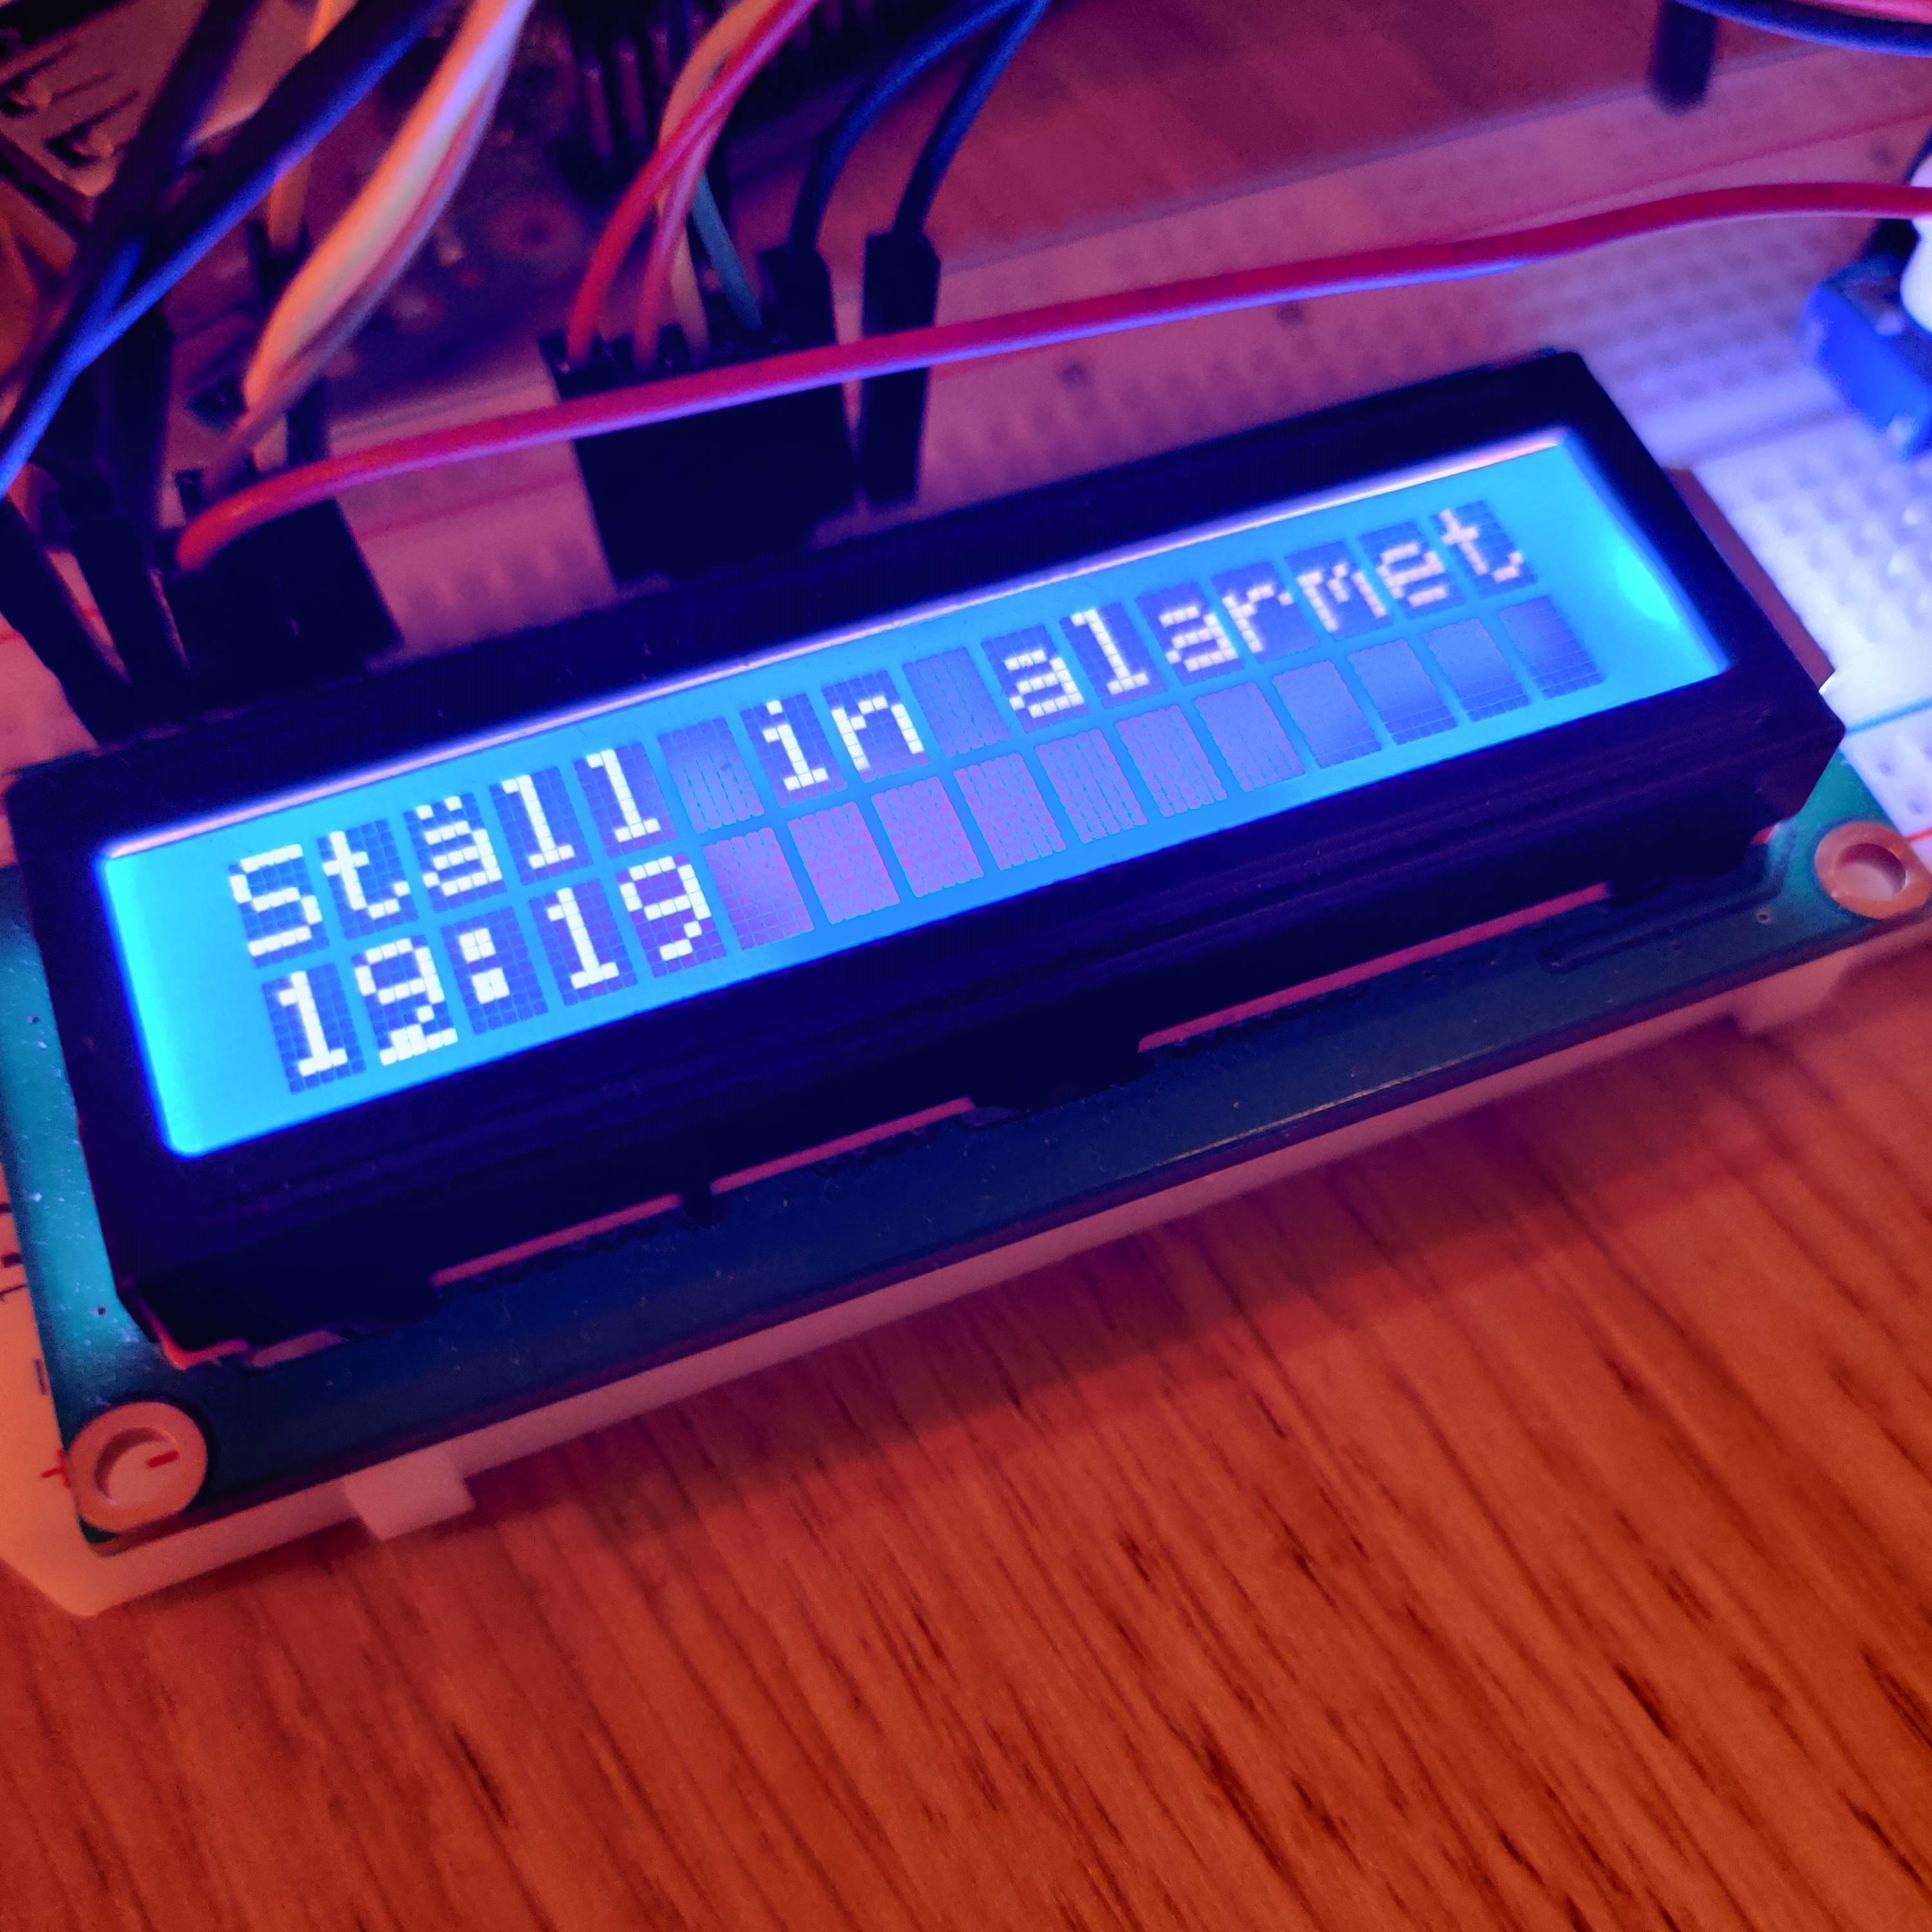
\includegraphics[width=0.9\textwidth]{bilder/stall alarm.jpg} % first figure itself
        \caption{Displayen vid inställning av alarmtid}
    \end{minipage}\hfill
    \begin{minipage}{0.30\textwidth}
        \centering
        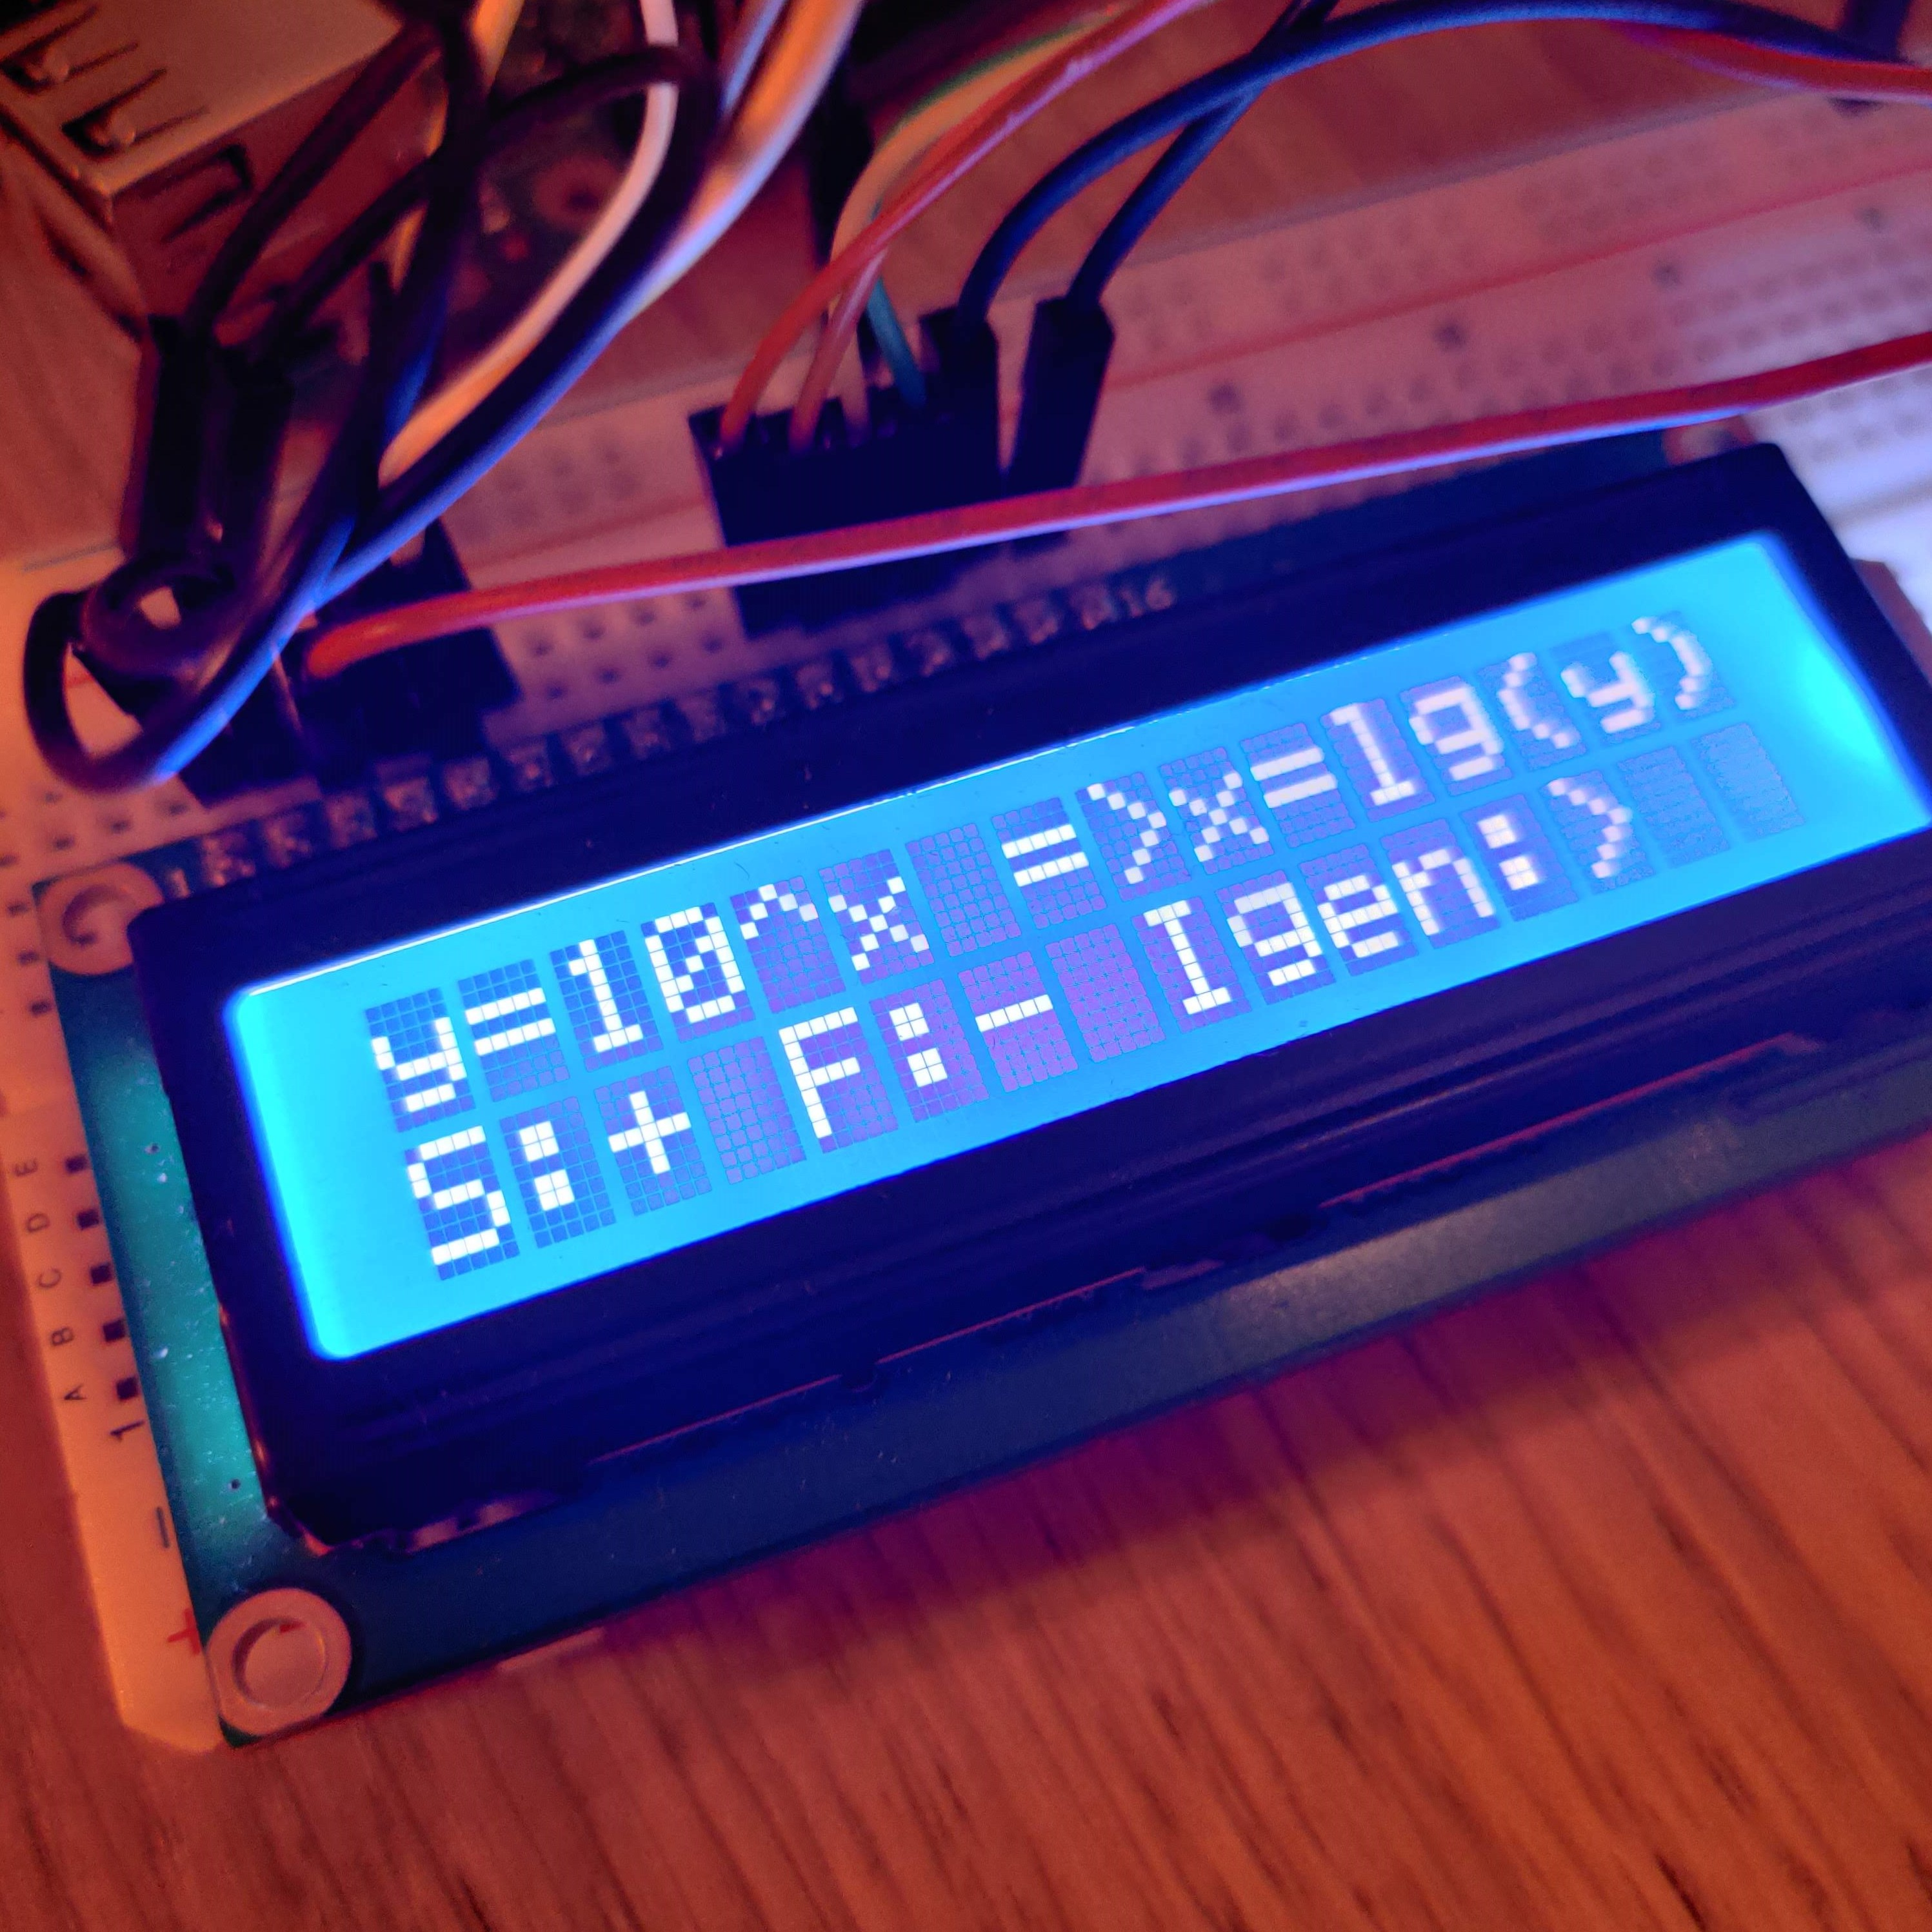
\includegraphics[width=0.9\textwidth]{bilder/sf fraga.jpg} % second figure itself
        \caption{En boolesk fråga}
    \end{minipage}\hfill
    \begin{minipage}{0.30\textwidth}
        \centering
        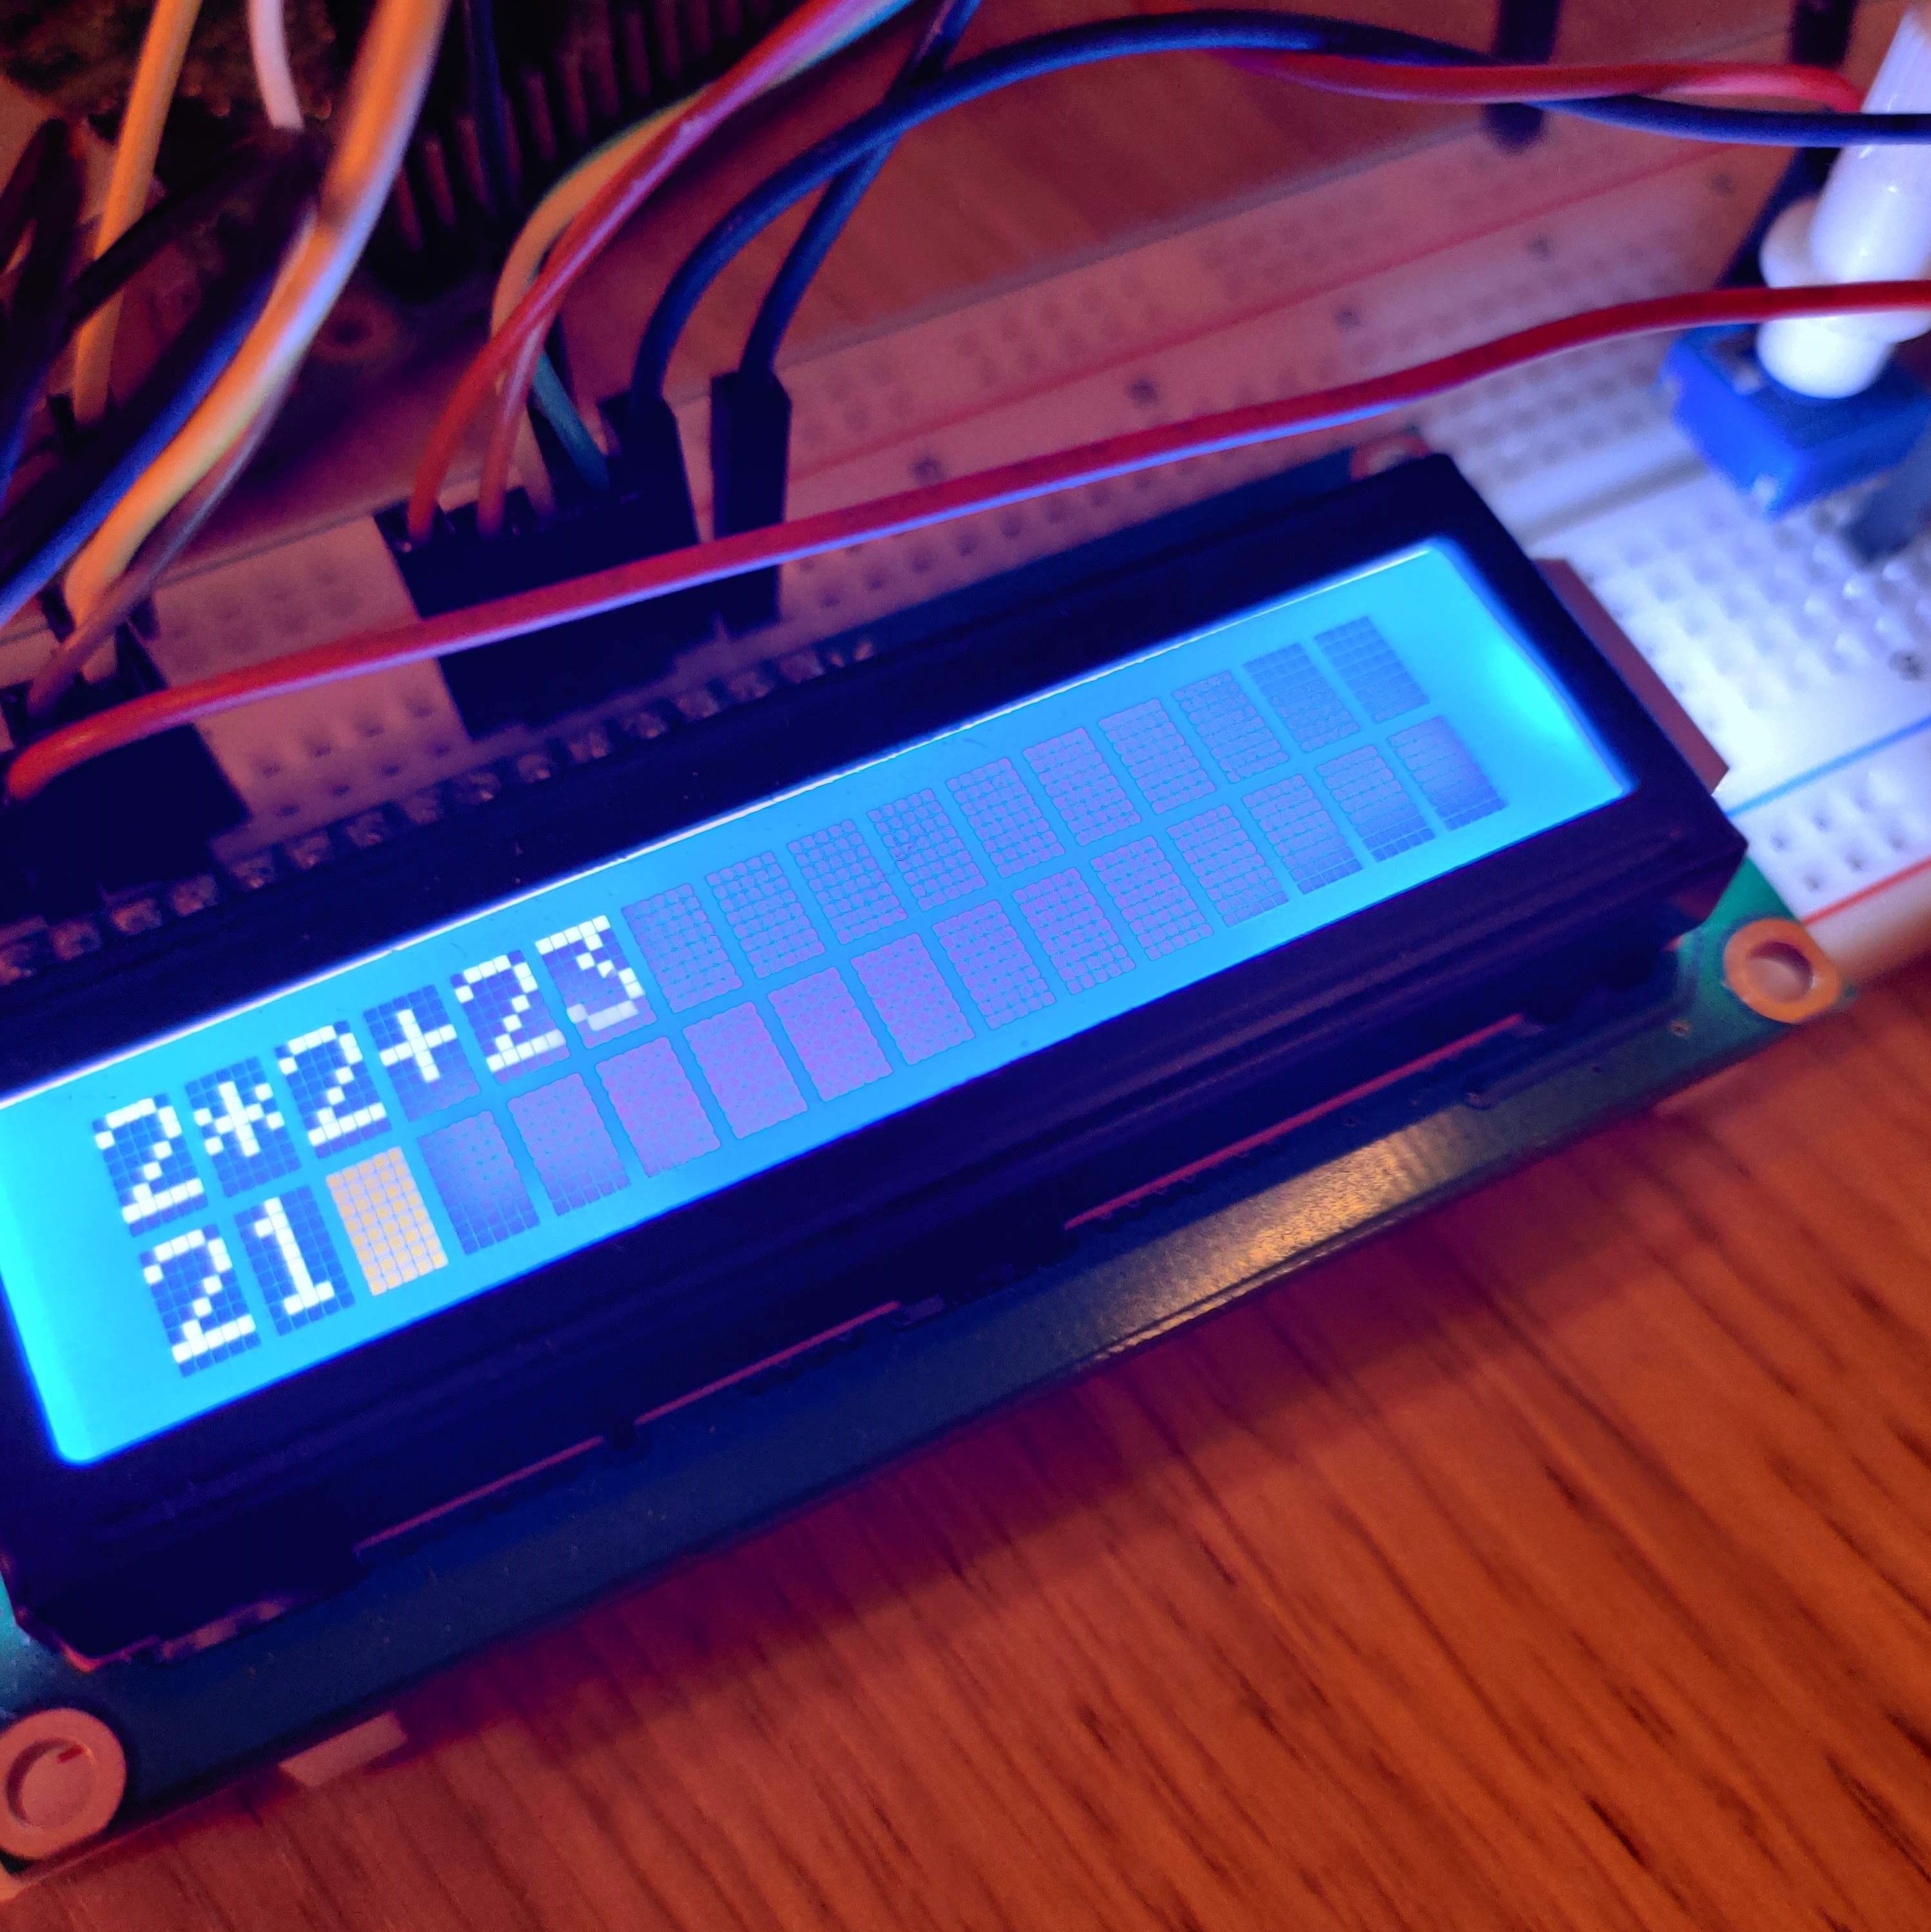
\includegraphics[width=0.9\textwidth]{bilder/ma alarm.jpg} % second figure itself
        \caption{En matematisk fråga}
    \end{minipage}
\end{figure}

%skrivet i python. Viktgia avsnitt bilder på skärmen för den kodbiten
%\subsection{Test}


    %\newpage
    
    \section{Diskussion}
    % {Hur skapas en smart väckarklocka?}
% {Hur ska en väckarklocka se till att vi verkligen går upp?)}

\subsection{Val av komponenter}
Kraven för datorn var att den skulle ha, lagringsutrymme för musik och frågor och minst 20 stycken stift. Stiften behövde både kunna ta emot och skicka ut signaler. Datorn behövde även kunna fjärrstyras med hjälp av SSH-teknik via en internetkabel. Datorn som uppfyllde dessa krav bäst var Raspberry Pi~3~B. Andra datorer som utvärderades var Raspberry Pi~3~A men den saknade ett nätverksuttag och hos Arduino Uno saknades ett användbart lagringsutrymme.

Angående högtalaren var tanken från början  att ha en liten högtalare kopplad till och driven av datorn. På grund av tidsbrist användes istället en högtalare kopplad med 3,5 mm kabel till datorns AUX-utgång.


\subsection{Kodens uppbyggnad}
Det som saknades i biblioteket \texttt{CHARLcd} var möjligheten att rulla text som är längre än 16 tecken. Detta löstes med denna metod: \begin{minted}{python}
if (len(string)>16): 
for x in range(len(string)-16):
    lcd.cursor_pos=(0,0)
    lcd.write_string(string[x:x+16])
    time.sleep(.5)}
\end{minted}
Om strängen består av fler än 16 tecken startas en for-loop som itereras för varje tecken som är för långt. För varje iteration hoppar strängen som skrivs ut ett steg till höger och pausar en halv sekund.  
%CHARLcd, knappar

%förklaring av vissa kodbitar med kod 




%\mint{python}|int 57|
%\mintinline{python}{for}
%\subsection{Ev. diskussion av resultatet från testnignen}
%Hjälper väckarklockan eller är den bara ett problem?

\subsection{Problem som uppstod under utvecklingsprocessen}
Under utvecklingen av väckarklockan uppstod några problem. Vissa var mjukvarurelaterade och några rörde hårdvaran.

Ett omfattande problem var att skärmen fortsatte att visa frågan istället för den nuvarande tiden efter korrekt besvarad fråga. Det visade sig att detta berodde på att en while-loop inte stängdes ner ordentligt. Detta löstes genom att att lägga in \emph{break}-kommandot i slutet av loopen som tvingade den att stoppa. 

I biblioteket \emph{pygame} som används för att spela upp alarmljudet fungerade inte kommandot för att stoppa alarmljudet. För att kringgå detta problem var biblioteket tvunget att återaktiveras vid varje alarmringning.

Ett problem som inte rörde programmet var att högtalaren inte kunde ansluta till datorn via blåtand. Istället behövdes den kopplas upp via kabel. En annan lösning skulle vara att koppla in en högtalare till datorns GPIO (se 4.4).

\subsection{Vidareutveckling av Proi Exypno}
En mer komplett och attraktiv väckarklocka kan fås genom att paketera produkten i ett skal. För att detta ska kunna göras måste ett kretskort skapas med alla komponenter fastlödda. Dessutom måste högtalaren som nu är kopplad med 3,5 mm kabel bytas ut mot en högtalare som är kopplad direkt till datorns utgångsstift. 

Väckarklockans mjukvara kan utvecklas så att andra typer av matematiska frågor läggs till, exempelvis på formen $a\cdot b - c\div d$.  Att fler frågor läggs in i frågebanken skulle också leda till en mer attraktiv produkt. För mer variation kan de booleska frågorna varieras med exempelvis flervalsfrågor, detta kräver dock fler knappar.
    \newpage
    
    
    \section{Referenser}
    \begin{hangparas}{.25in}{1} 
BoredPanda. (2011). ''20 Annoyingly Creative Alarm Clocks''. Hämtad 20-02-10 från \url{www.boredpanda.com/20-annoyingly-creative-alarm-clocks/}.
\smallskip

%Bargen, Danilo. (2018). ''Welcome to RPLCD’s documentation!''. Hämtad 19-10-30 från \url{https://rplcd.readthedocs.io/en/stable/}.

%Circuit Basics. (u.å.). ''How to setup an LCD on the Raspberry Pi and program it with Python''. Hämtad 19-10-30 från \url{www.circuitbasics.com/raspberry-pi-lcd-set-up-and-programming-in-python/}.
%\smallskip

%Pygame documentation. (u.å.). ''pygame.mixer''. Hämtad 20-01-06 från \url{www.pygame.org/docs/ref/mixer.html}.
%\smallskip

%Raspberry Pi HQ. (2018). ''Using a push button with Raspberry Pi GPIO". Hämtad 19-10-30 från \url{www.raspberrypihq.com/use-a-push-button-with-raspberry-pi-gpio/}.
%\smallskip

Roitmann, Eva. (2017). ''To Snooze or Not to Snooze: The Truth About the Snooze Button''. Hämtad 20-02-08 från \url{https://blog.withings.com/2017/03/16/to-snooze-or-not-to-snooze-the-truth-about-the-snooze-button/}.
\smallskip

TT. (2013, 8 april). Snooza kan göra mer skada än nytta. \textit{Dagens Nyheter.} Hämtad från \url{https://www.dn.se/nyheter/vetenskap/snooza-kan-gora-mer-skada-an-nytta/}.
\end{hangparas}

    \newpage
    \section{Bilagor}
        \subsection{Formulärsvar}
            \label{sec:svar}
            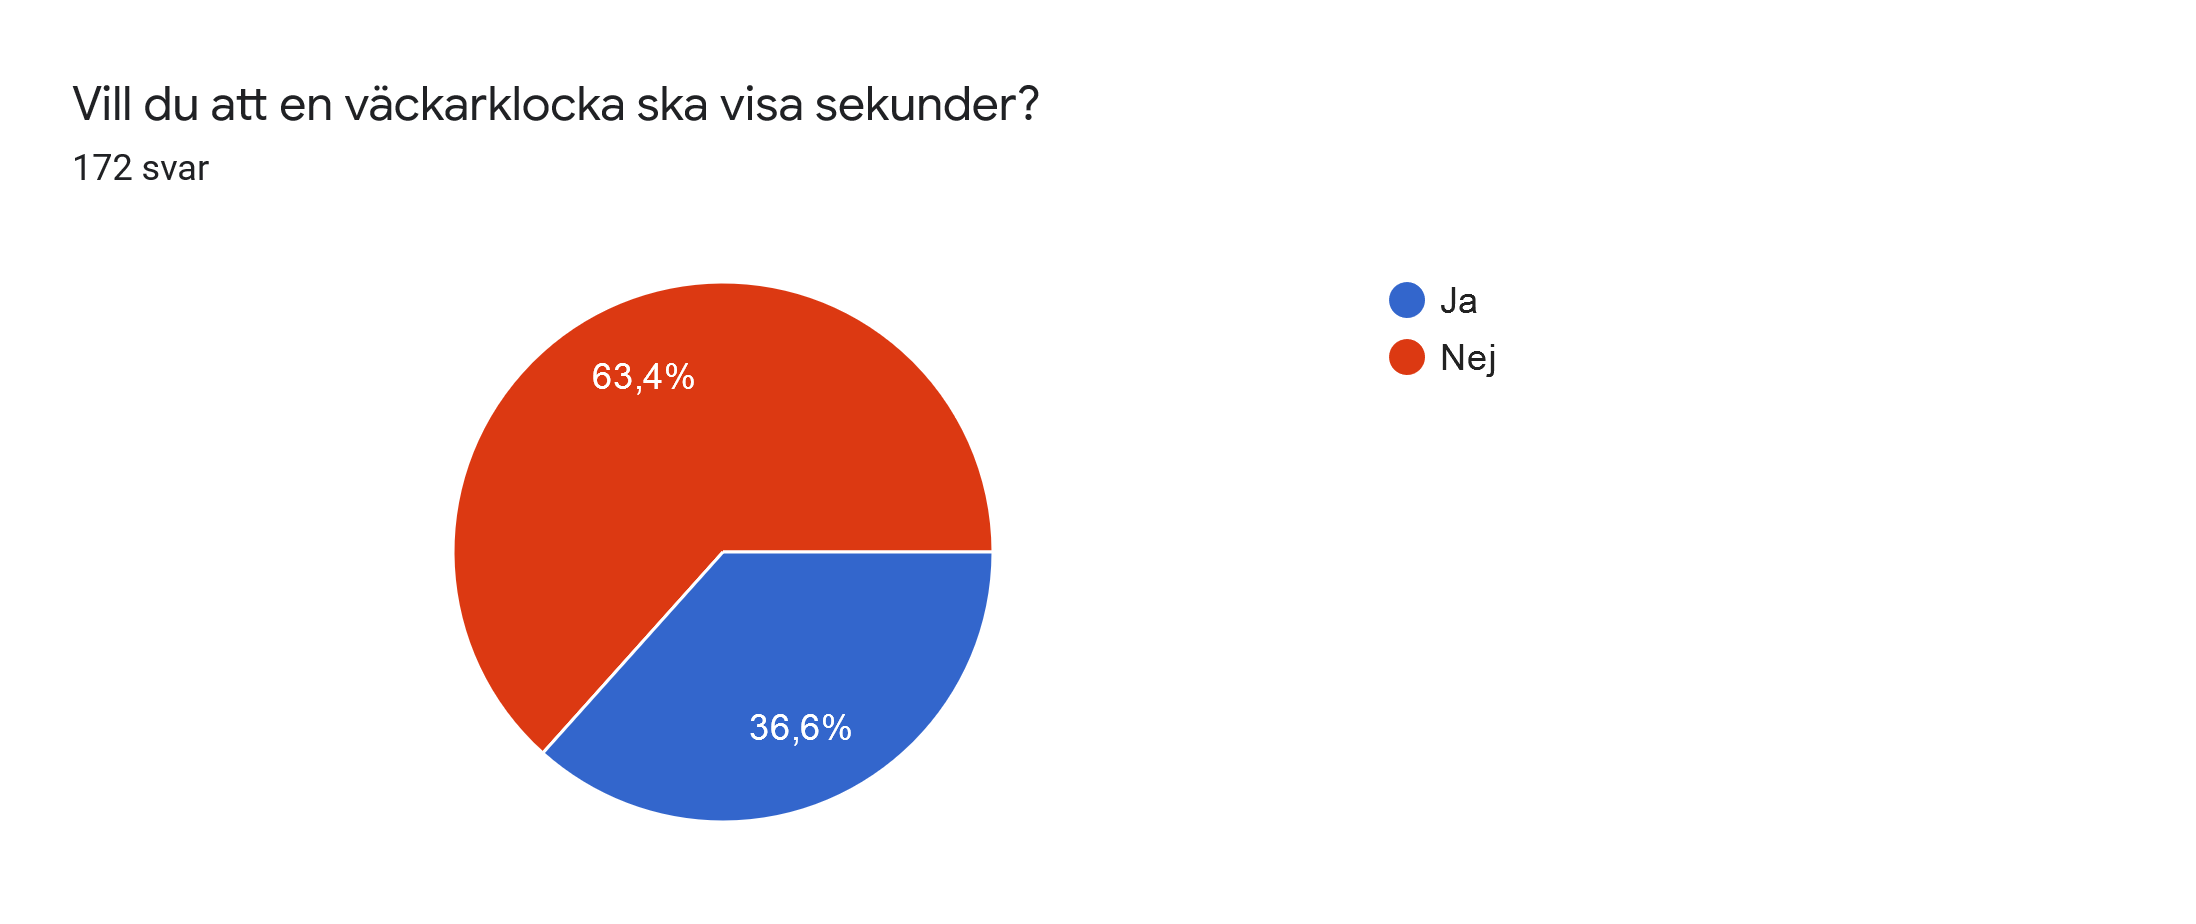
\includegraphics[scale=0.35]{fraga1.png}
            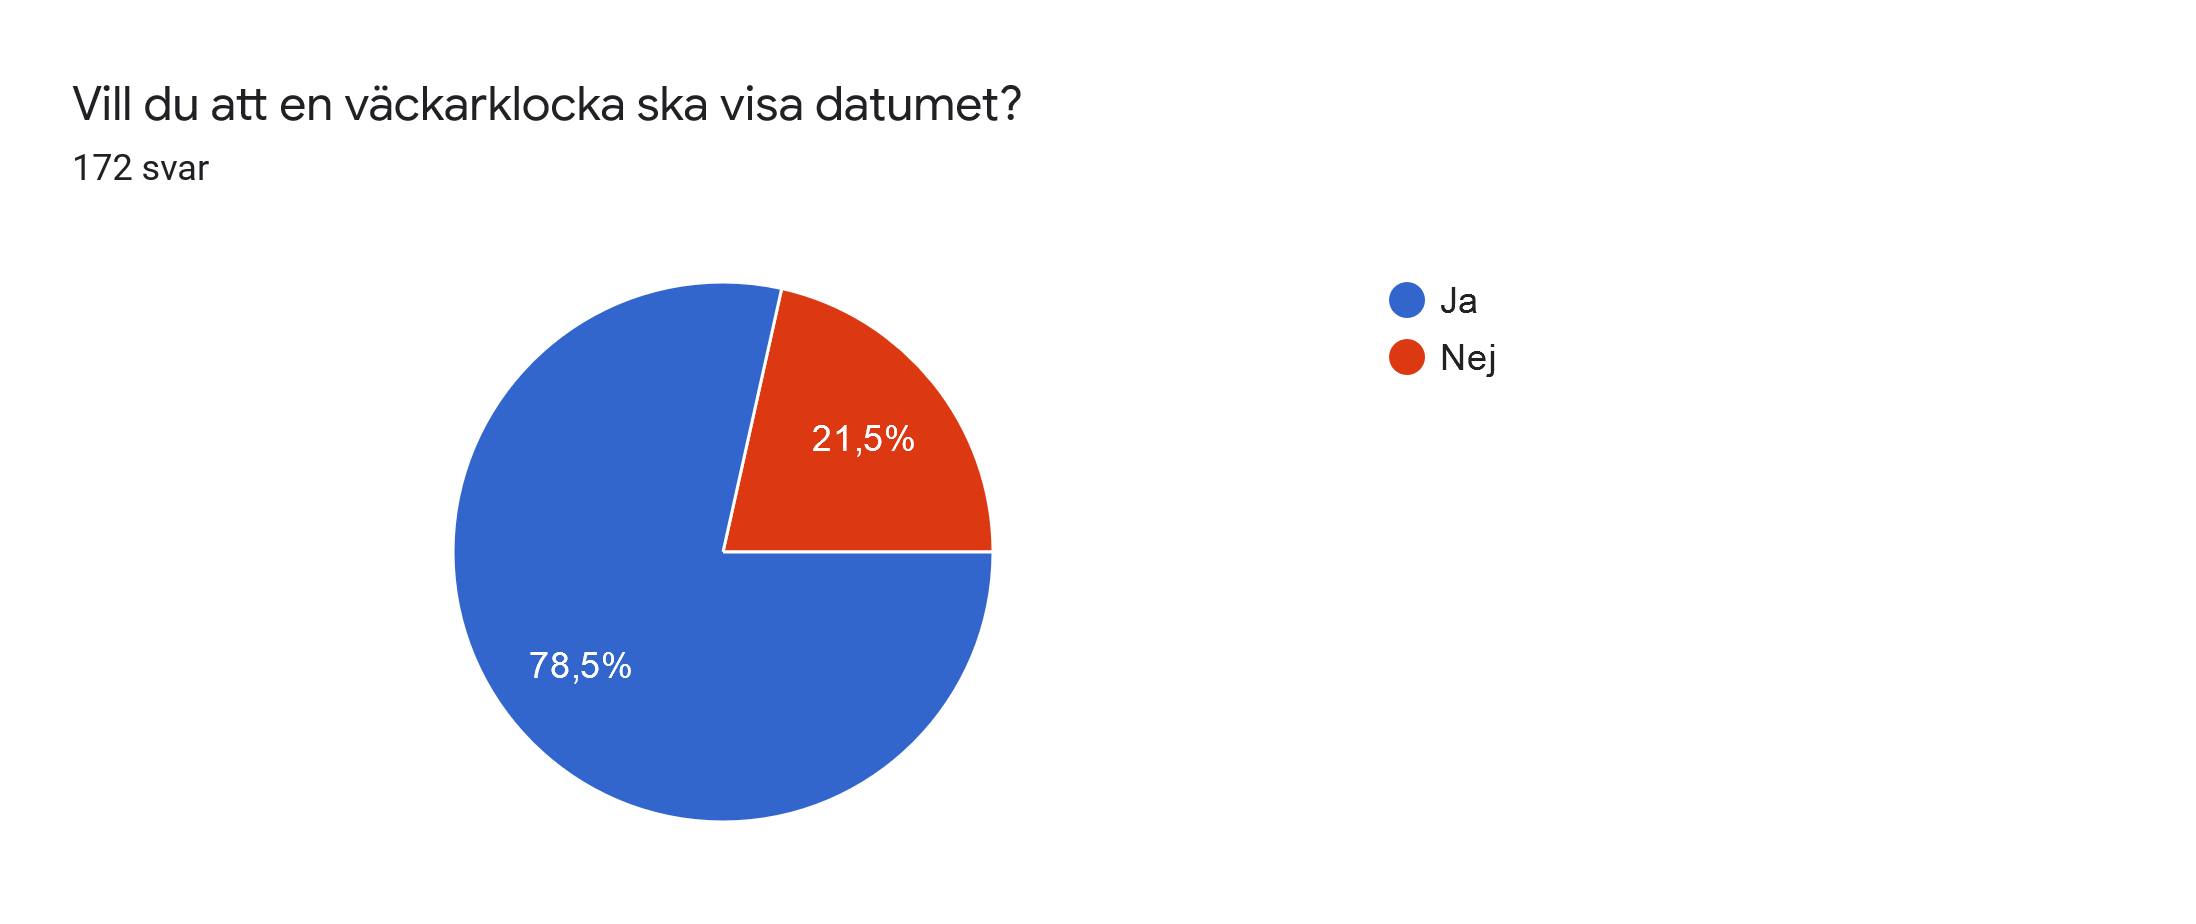
\includegraphics[scale=0.35]{fraga2.png}
            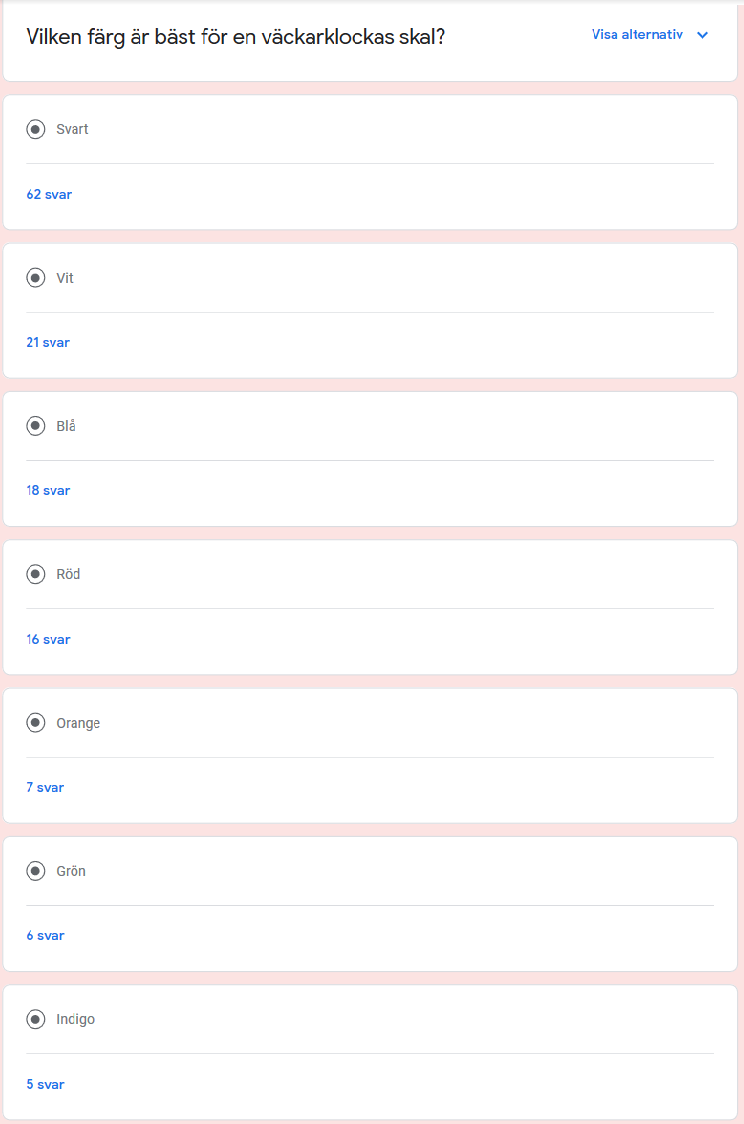
\includegraphics[scale=.7]{fraga1ny.png}            
        %\subsection{Budget}
         %   \label{sec:budget}
          %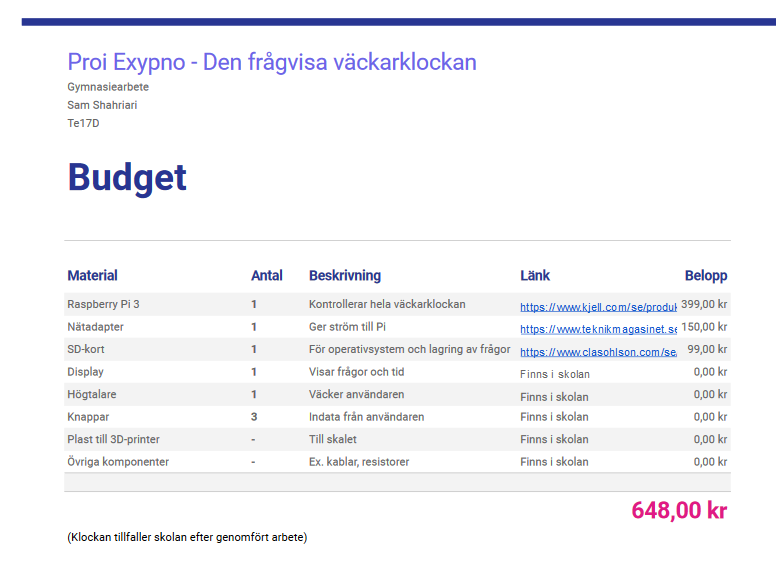
\includegraphics[scale=0.7]{budget.PNG}
        \subsection{Pseudokod}
            \label{sec:psuedo}
            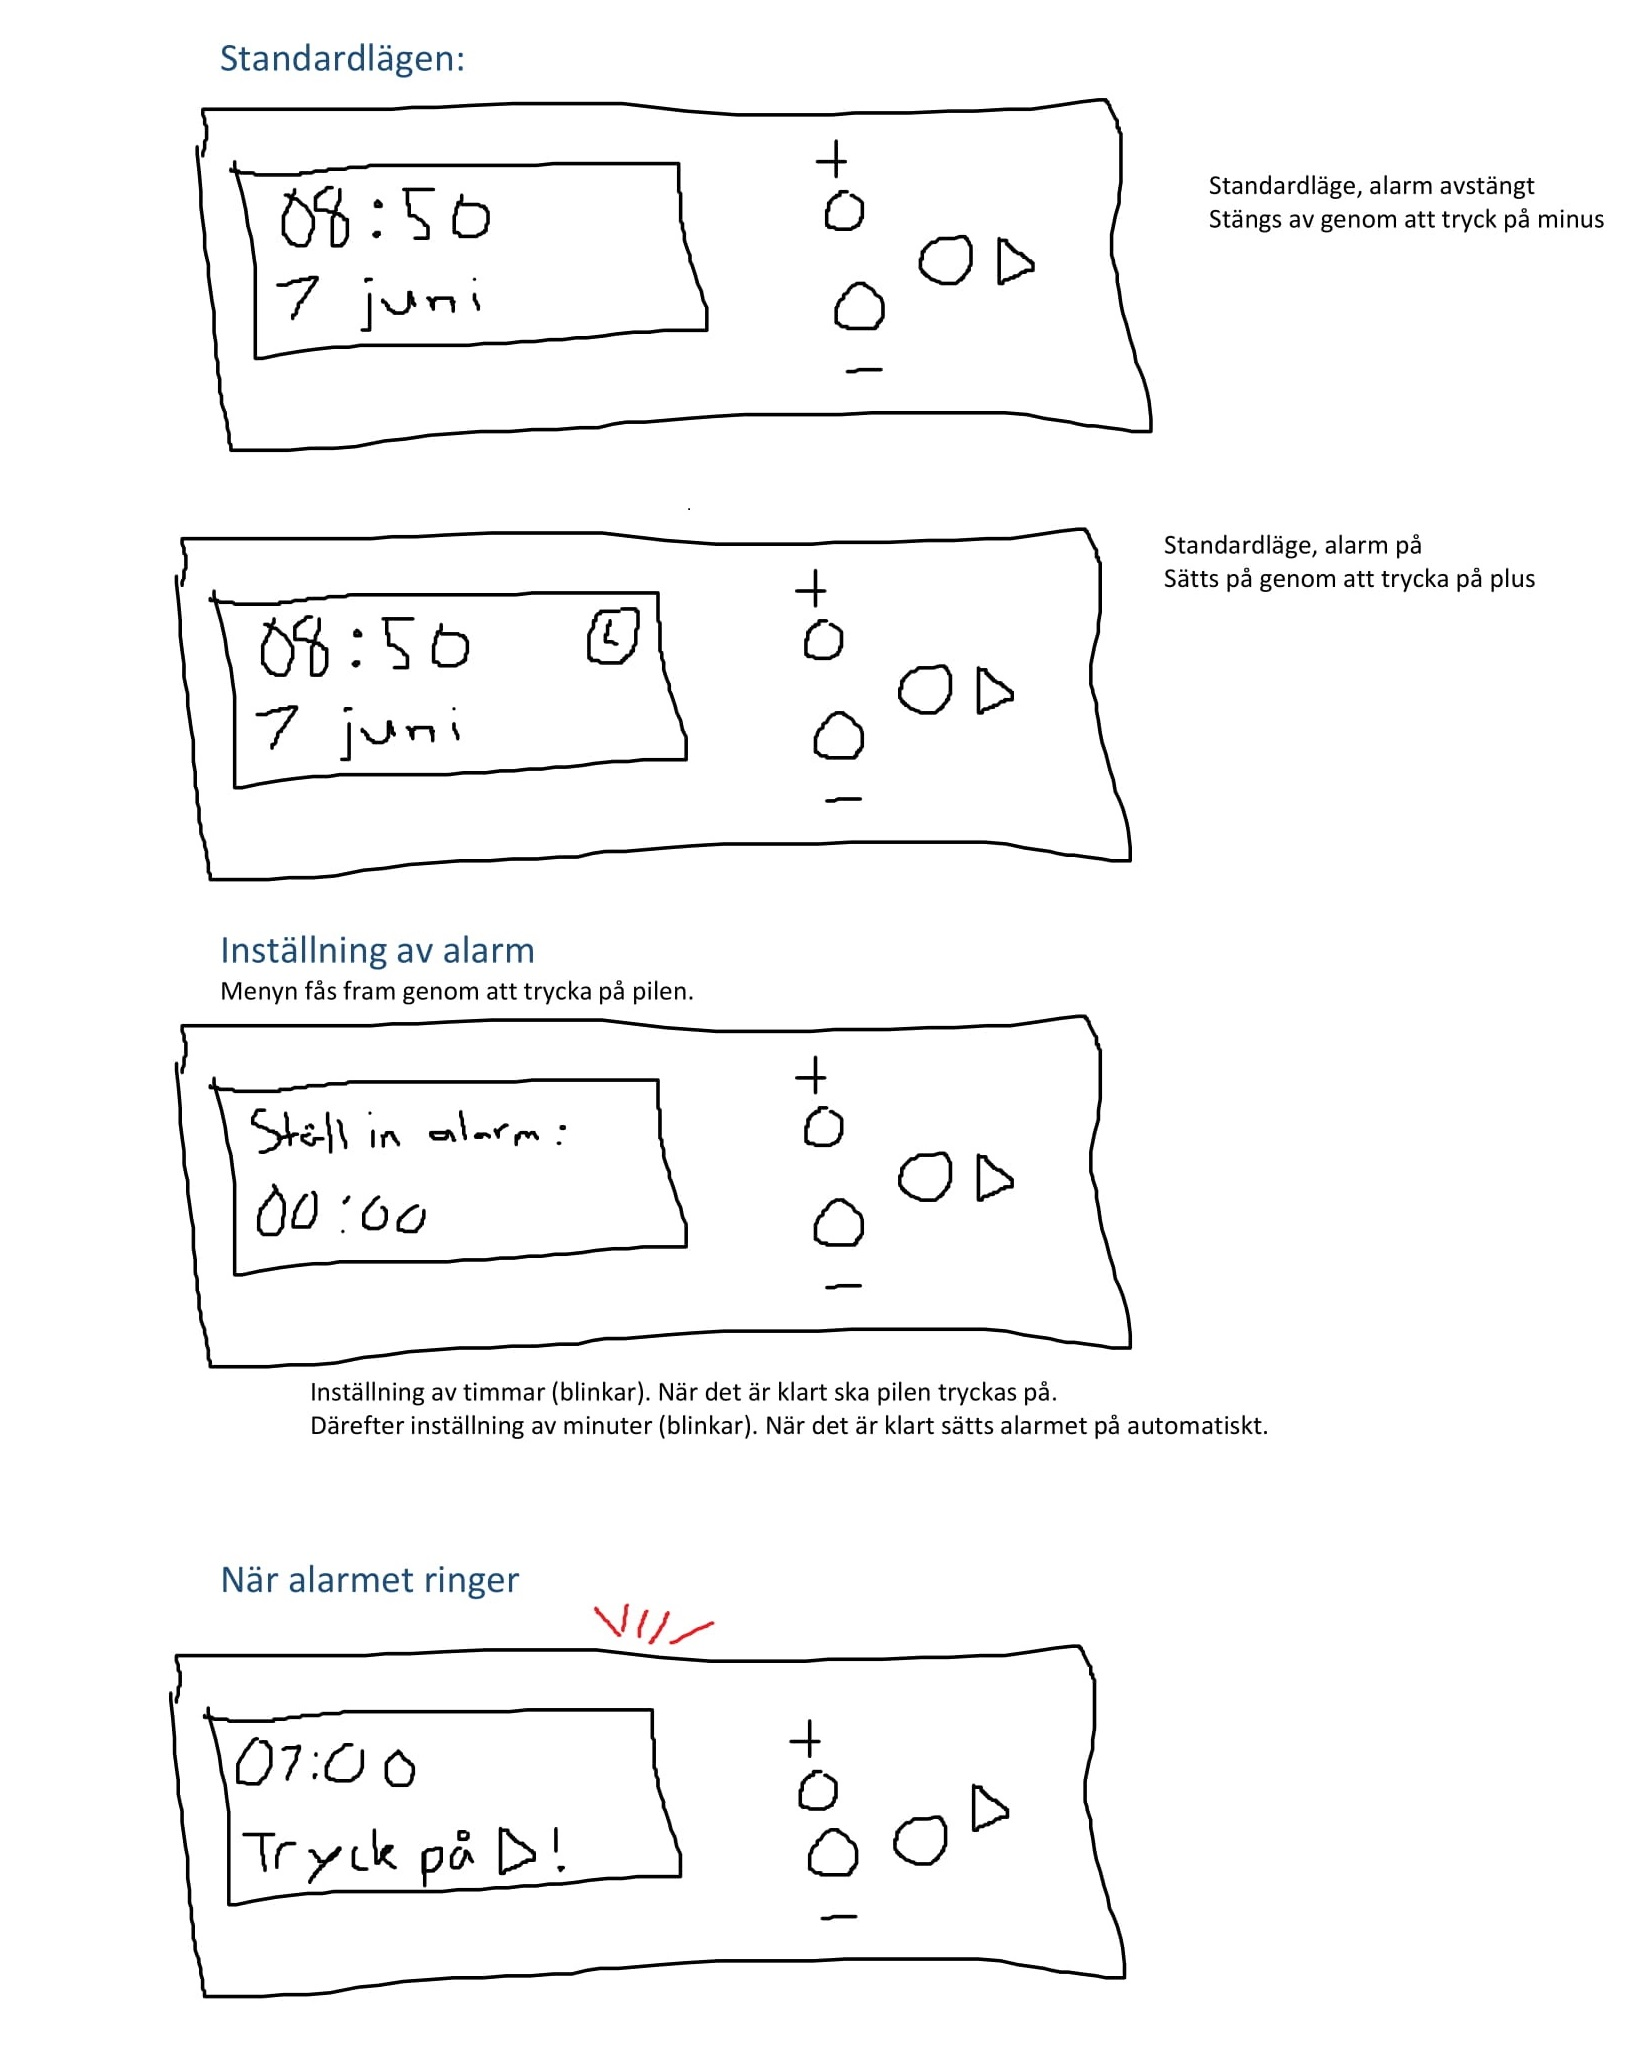
\includegraphics[scale=0.35]{Pseudokod-1.jpg}
            \newpage
            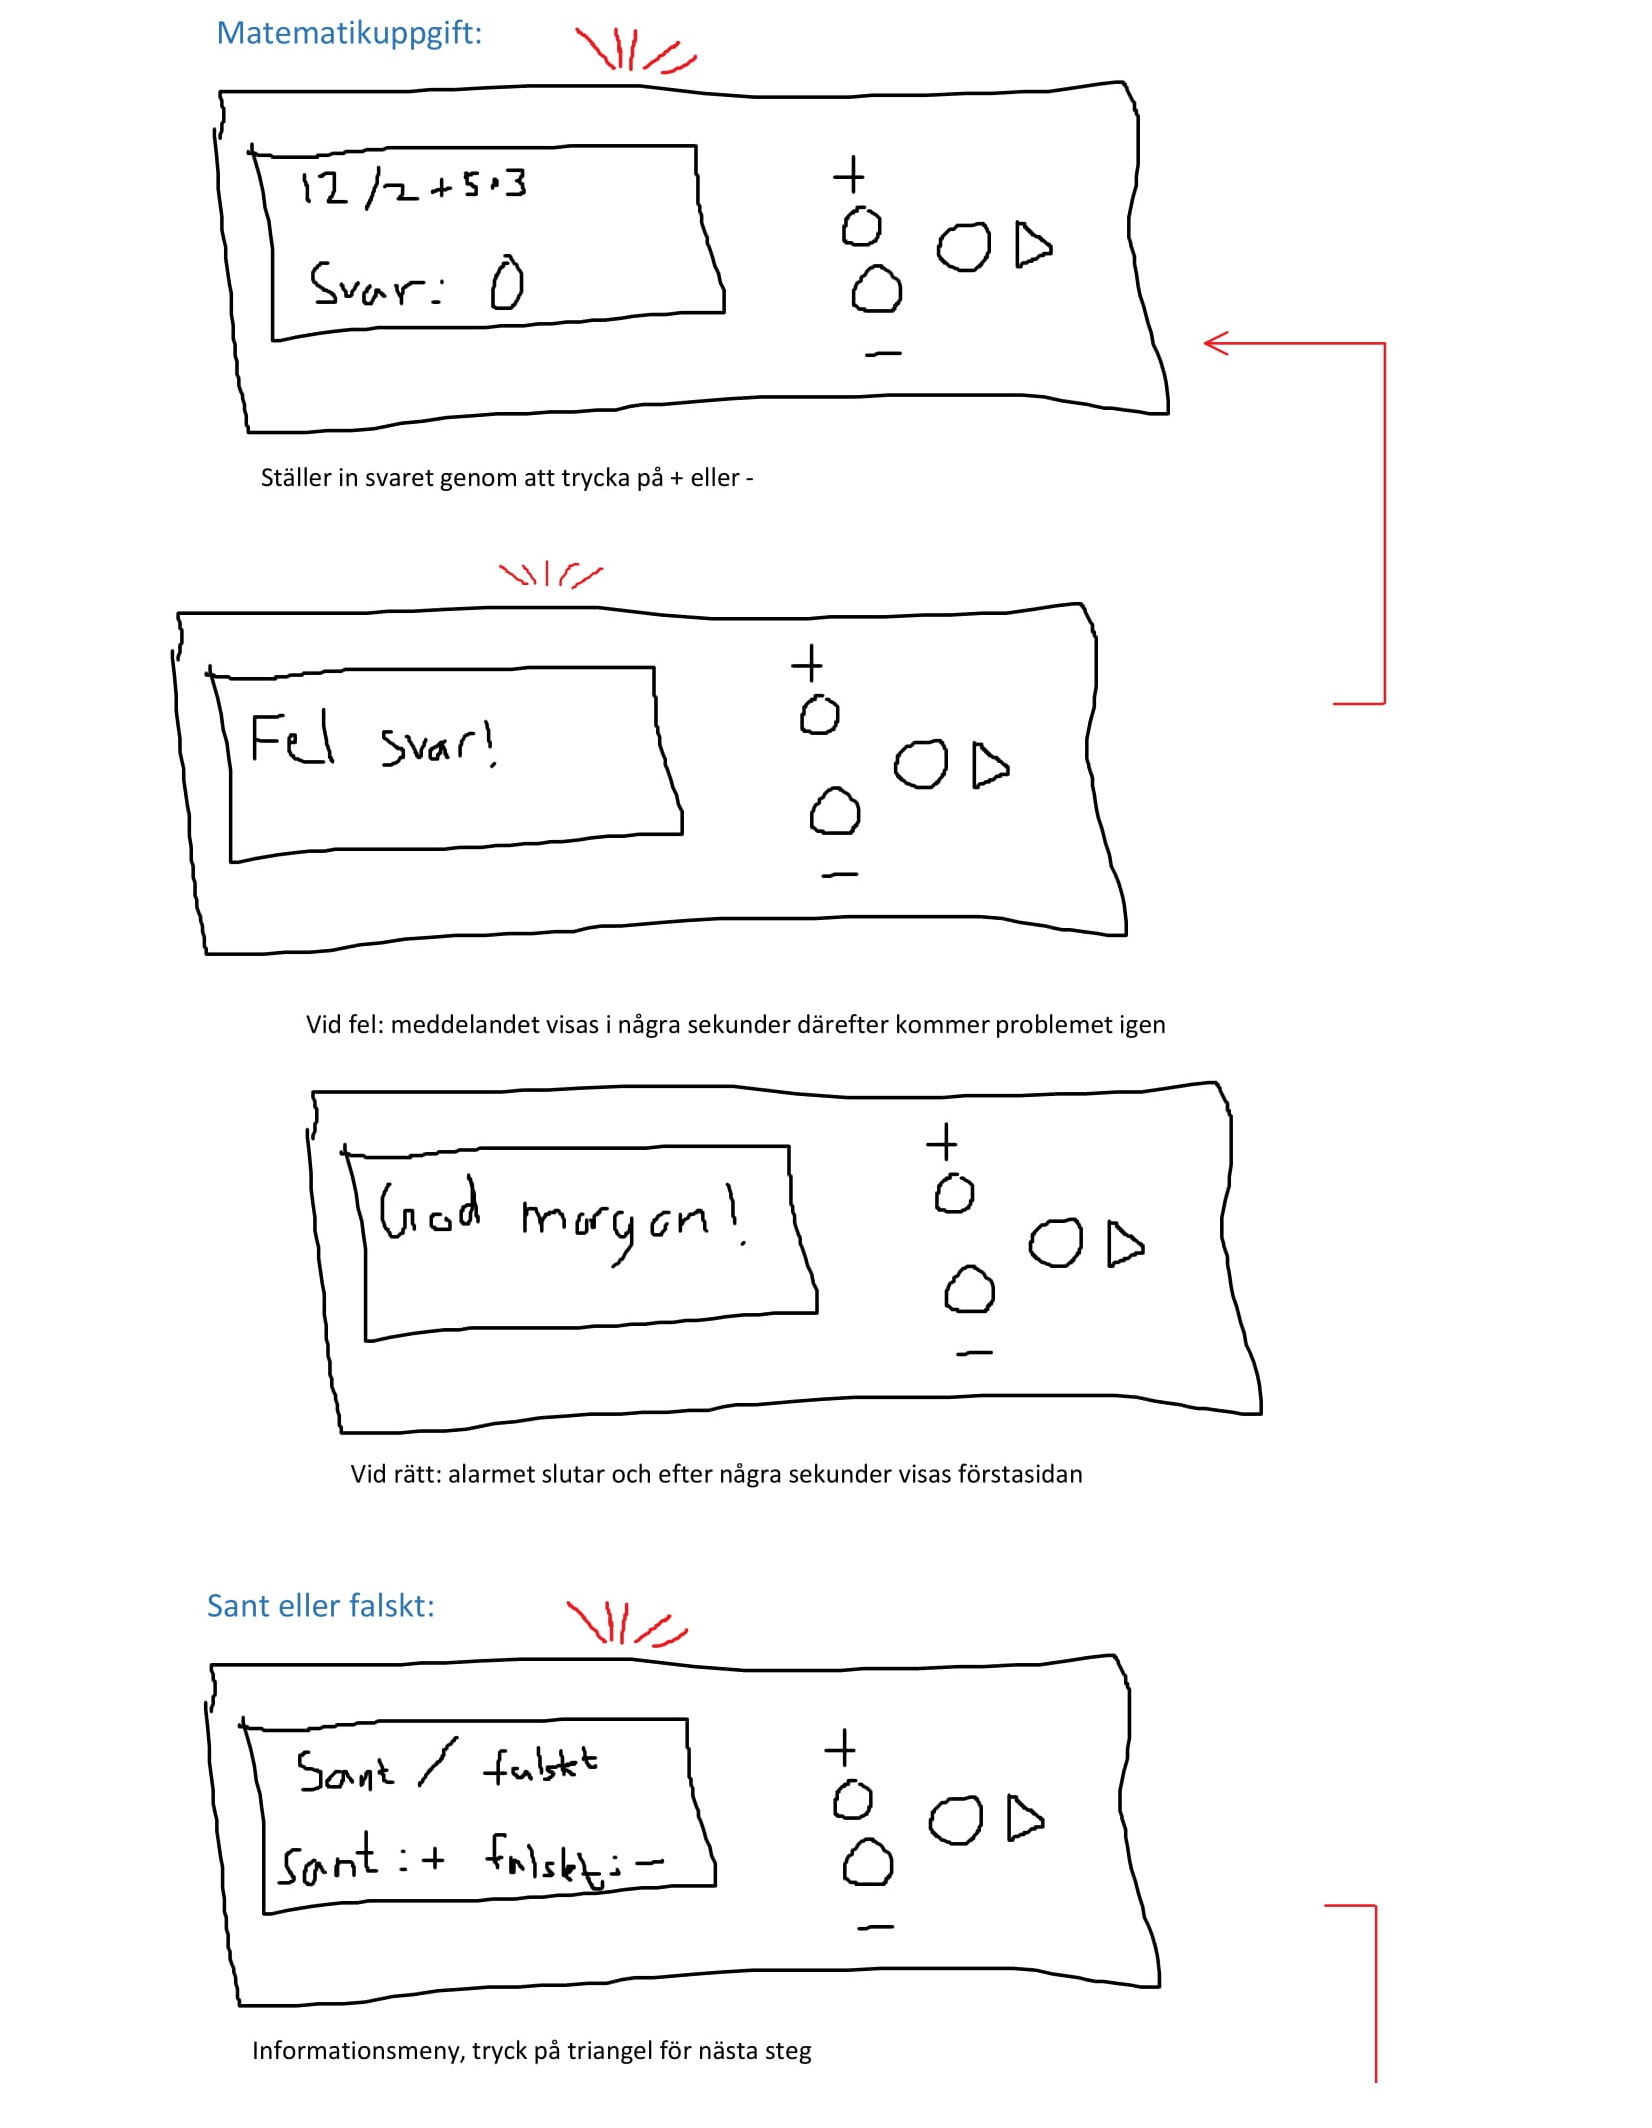
\includegraphics[scale=0.35]{Pseudokod-2.jpg}
            \newpage
            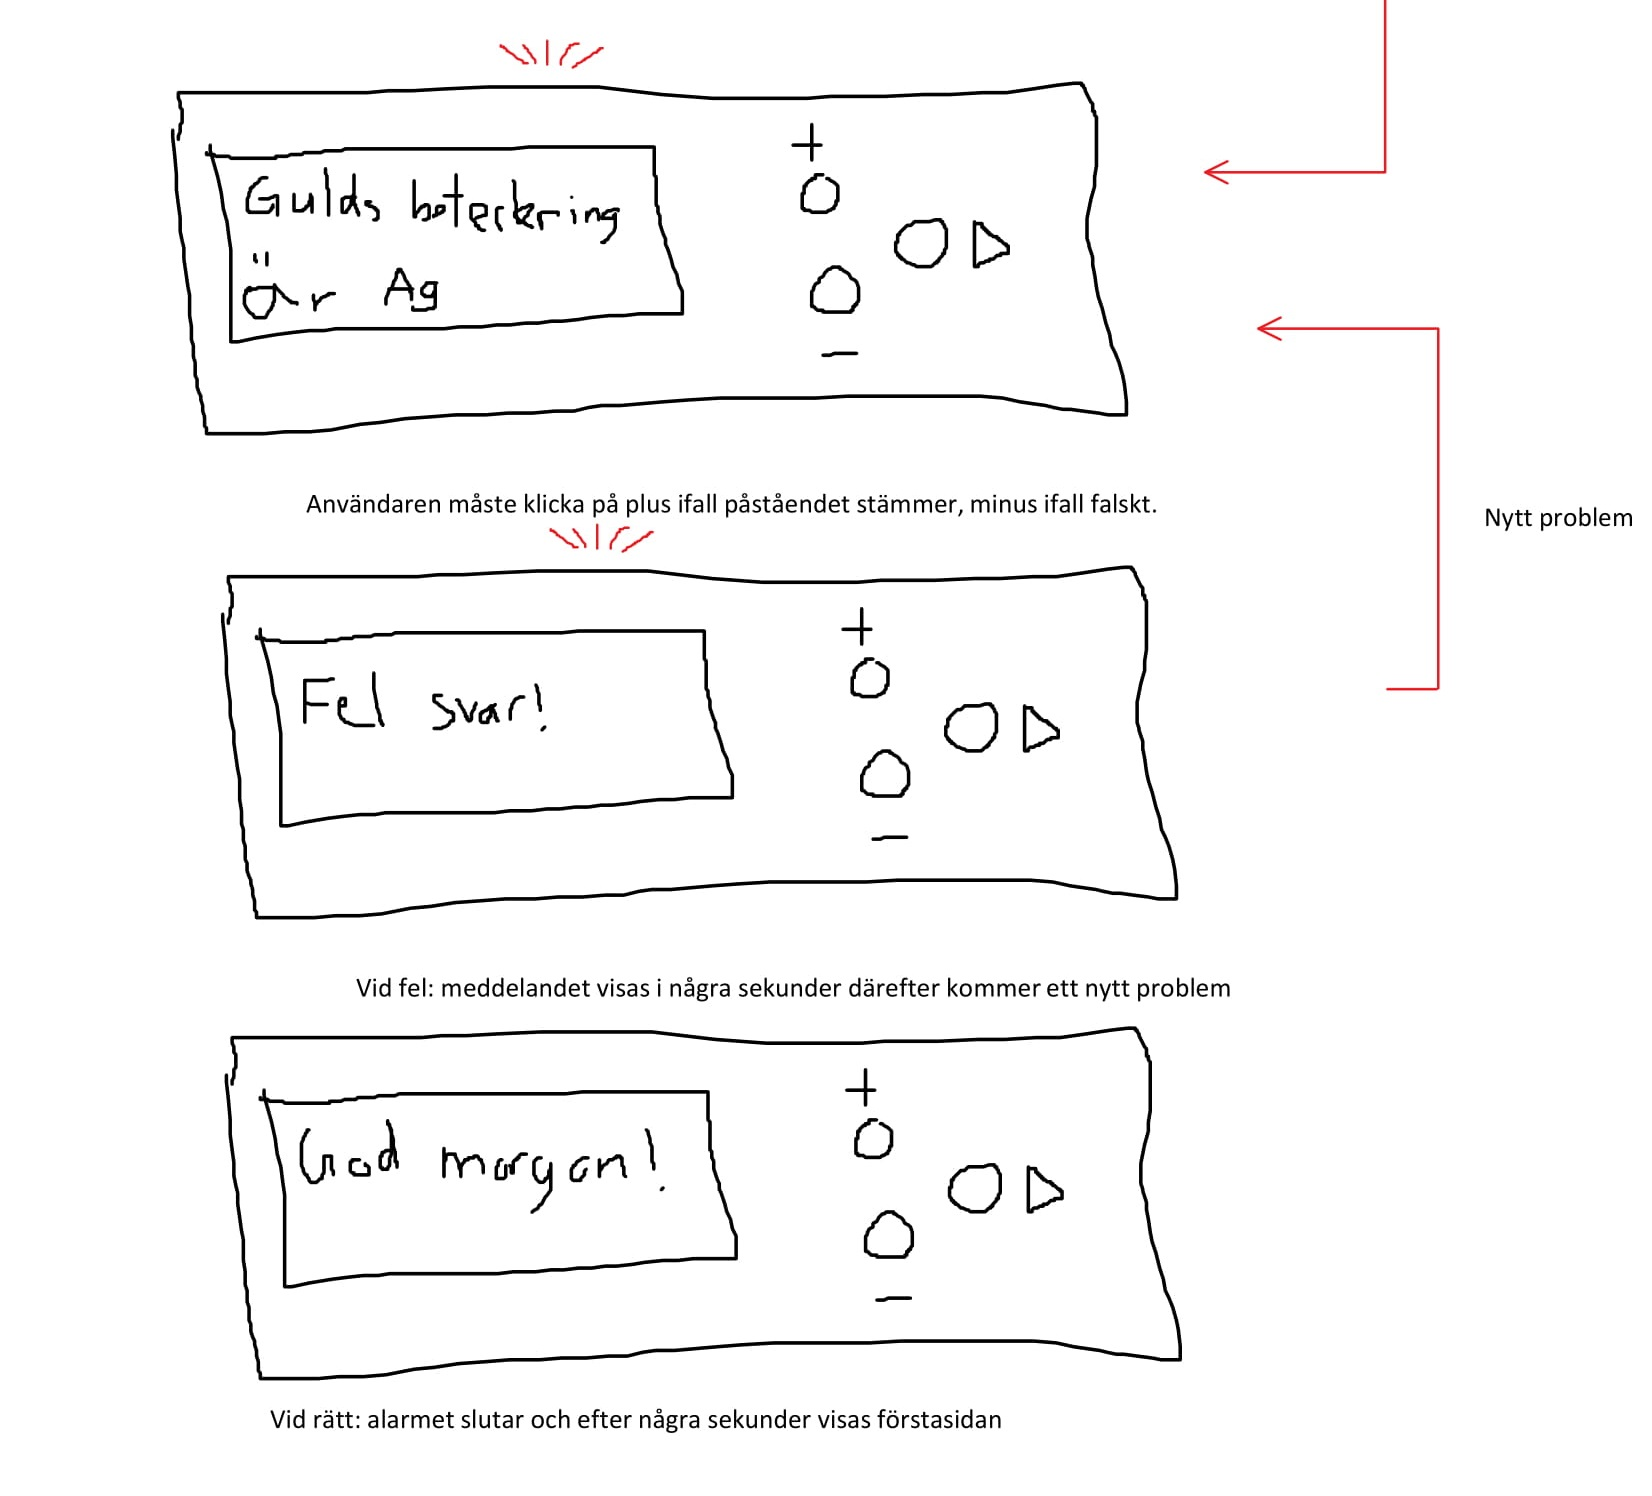
\includegraphics[scale=0.35]{Pseudokod-3.jpg}
            \newpage
            
        \subsection{Kod}
        \label{sec:kod}
            \tiny{\inputminted{python}{lcd.py}}
            \newpage
        \subsection{fragor.txt}
        \label{sec:fragor}
            \normalsize{\begin{verbatim}
Guld har beteckningen Ag
0
f(x)=5x^2+2x => f'(x)=10x+2
1
f(x)=5x^2+2x <=> f'(x)=10x+2
0
Elektronikkomponenten 555 ar en AND-gate
0
En triangels vinkelsumma ar alltid 180*
0
373 ar ett primtal
1
y=10^x =>x=lg(y)
1
En parabel ar en tredjegradsfunktion
0
En n:te gradsfunktion har alltid n st losningar
1
|-5+3|=8
0
sqrt(-1)=j
0
f(x)=sin(cos(x)) => f'(x)=cos(cos(x))*sin(x)
0
\end{verbatim}}
            \newpage
        \subsection{Kretsschema}
        \label{sec:krets}
            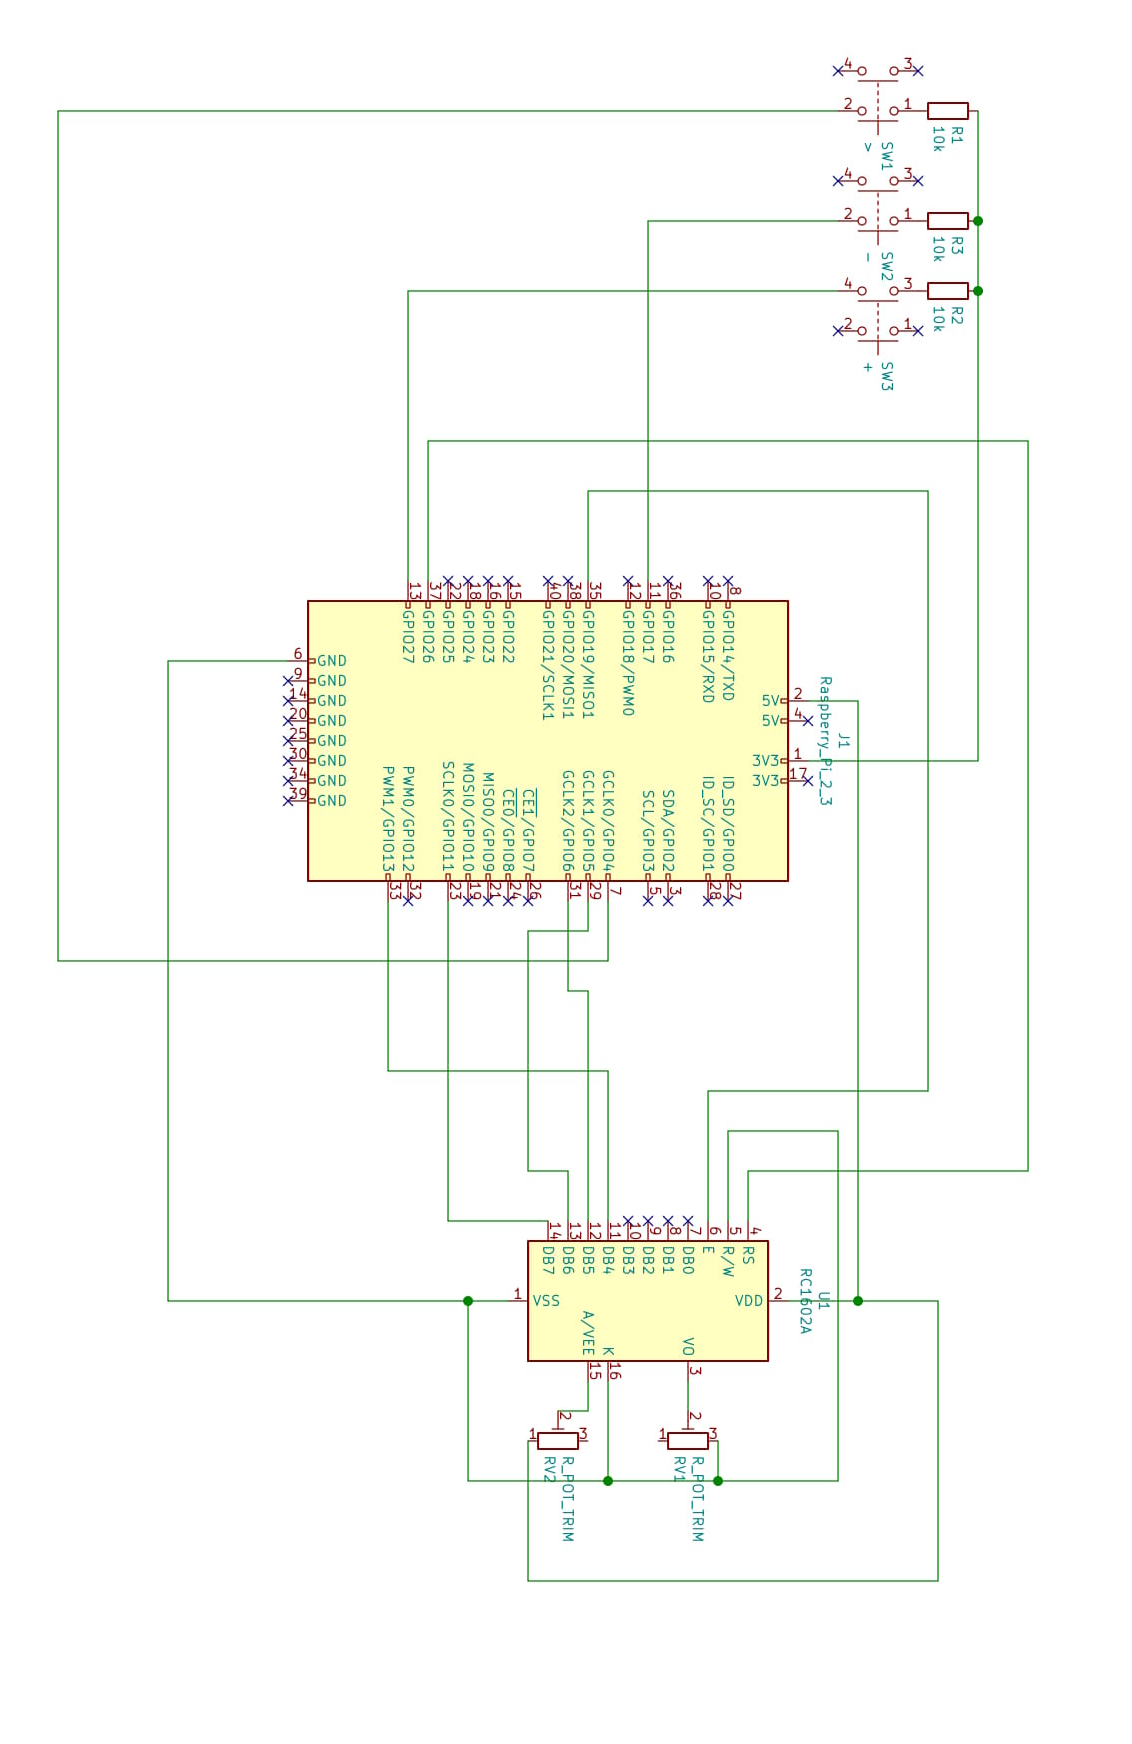
\includegraphics[scale=0.4]{krets.png}

\end{document}
